\documentclass[10pt,a4paper,appendixprefix,pdfusetitle,twocolumn,draft]{scrbook}

\usepackage{svn}
\SVN $Revision: 295 $
\SVN $Author$
\SVN $Date$
\SVN $URL: https://qetesh.gwerder.net/svn/mailvortex/doc/mailvortex.tex $
\SVN $Id$

\makeatletter
\def\title#1{\gdef\@title{#1}\gdef\thetitle{#1}}
\usepackage{lipsum}

\title{MessageVortex}
\gdef\thesubtitle{Transport Independent Messaging Anonymous to \nth{3} Parties}
\subtitle{\thesubtitle}
\author{Martin Gwerder (06-073-787)}
\date{\SVNDate}
\gdef\myabstract{In this paper we introduce an unobservable message annonymisation protocol, named MessageVortex. It is based on the zero trust principle and a distributed peer-to-peer (P2P) architecture and avoids  central aspects such as fixed infrastructures within a global network. It scores over existing work by blending its traffic into suitable existing transport protocols, thus making it next to impossible to block it without significantly affecting regular users of the transport medium. It furthermore requires no protocol specific infrastructure in public networks and allows a sender to control all aspects of a message such as degree of anonymity, timing, and redundancy of the message transport without disclosing any of these details to the routing or transporting nodes.}
\makeatother

% enable graphics inclusion
\usepackage[final]{graphicx}

\usepackage{hyperxmp}

\usepackage{xcolor}

\usepackage{xstring}

\usepackage{pdfsync} 

\usepackage{MnSymbol} % required for the arrow

%\usepackage{underscore}

% titlepage geometry change
\usepackage[paper=a4paper,top=2cm,bottom=2cm,inner=2cm,outer=2cm]{geometry}% http://ctan.org/pkg/geometry

\usepackage{scrhack}

\usepackage[autocite=superscript,
            backref=true,
            backend=bibtex,
            hyperref=true,
            url=true,
            isbn=true,
            maxcitenames=3,
            maxbibnames=100,
            block=none,
            sorting=anyt]{biblatex}

%\bibstyle{alphadin}
\addbibresource{messageVortex}
\addbibresource{inc/bib/unclassified/Anonbib/anonbib}
\usepackage{csquotes}

% For Multipage listing in appendix
\usepackage[final]{listings}
\usepackage{caption}
\usepackage[framemethod=tikz]{mdframed}
\usepackage[many]{tcolorbox}
\tcbuselibrary{listings}

% enable raggedright in tables
\usepackage{array}
% for diagonal divided cells in tables
\usepackage{makecell}
\renewcommand\theadfont{\bfseries}

% footnotes for tables
\usepackage{tablefootnote}
%\makesavenoteenv{tabular}

% enable placement of floating images
\usepackage{float}

%enable page spanning tables
\usepackage{supertabular}

% enable superscript  for 1st, 2nd, 3rd etc.
\usepackage[super]{nth}

%enable hypelinks
\usepackage[pdftex]{hyperref}
\makeatletter
\hypersetup{
  hidelinks,
  pdftitle={\thetitle},
  pdfpagelayout=TwoPageRight,
  bookmarks=true,
  hyperindex=true,
  hyperfigures=true,
  pdftex=true,
  pdfpagelabels=true,
  pdfstartview=Fit,
  pdfauthor={\author},
  pdftitle={\thetitle\\\small\thesubtitle},
  pdflang=en,
  pdfsubject={\myabstract},
  pdfkeywords={Messaging, Anonymity, SMTP, MIME, S/MIME, POP3, IMAPv4, Message Vortex},
  pdfcontactemail={martin.gwerder@fhnw.ch},
  pdflicenseurl={http://creativecommons.org/licenses/by-nc-nd/3.0/ch/},
  pdfcopyright={"Creative Commons Attribution-NonCommercial-NoDerivatives 3.0 Switzerland" (CC BY-NC-ND 3.0 CH)}
}
\makeatother

% for PDF/A generation
%\usepackage[a-3b]{pdfx}



% Link above tables and figures
%\usepackage[hypcap]{caption}

% support repetitive footnotes
\usepackage{fixfoot}

% Document annotations
\usepackage[nomargin]{fixme}
\fxsetup{layout=pdfnote}

%enable attached files
\usepackage{attachfile}

%enable word separation
\usepackage[english]{babel}

% enable nice references
\usepackage{fancyref}

% For abstracts
\makeatletter
\newenvironment{abstract}{%
	\if@twocolumn
	\section*{\abstractname}%
	\else
	\small
	\begin{center}%
		{\bfseries \abstractname\vspace{-.5em}\vspace{\z@}}%
	\end{center}%
	\quotation
	\fi}
{\if@twocolumn\else\endquotation\fi}
\makeatother

% Enable indexes
\usepackage{makeidx}
\makeindex 

% format appendix
\usepackage[titletoc,page,title]{appendix} %enable appendix 

% citations
%\usepackage{cite}

% set numbering for subsubsections
\usepackage{tocstyle}
\setcounter{secnumdepth}{3}
\setcounter{tocdepth}{4}

% Sans serif font for the whole document
\renewcommand{\familydefault}{\sfdefault}
\usepackage[T1]{fontenc}
\usepackage{times}

\usepackage{amsmath}

% No paragraph indentation
\setlength\parindent{0pt} 
\setlength\parskip{6pt} 

% For coments and similar
\usepackage{verbatim}

% For Page background color
\usepackage{afterpage}
\usepackage{xcolor} 


\usepackage{tabularx}
\usepackage{multirow}

% XMP support 
\RequirePackage{xmpincl}
\includexmp{messageVortex}

% Required for definitions environment
\usepackage{hanging}
\usepackage{ragged2e}
\newenvironment{entry}{\par\leavevmode\hangpara{1.5mm}{1}\ignorespaces}{\RaggedRight\par}
\newcommand*{\mainentry}[2]{{\bfseries{#1\label{def:#1}}}~#2\par}
\newcommand*{\subentry}[2]{\par~\begin{tabular}{p{\textwidth-.6cm}@{}}{\bfseries{\itshape{#1\label{def:#1}}}}~#2\end{tabular}}

\newcommand*{\defref}[1]{\hyperref[def:#1]{#1}}
\title{MessageVortex}
\subtitle{Transport Independent Messaging anonymous to \nth{3} Parties}
\author{Martin Gwerder (06-073-787)}
\date{\SVNDate}

%\hypersetup{pdfinfo={
%Subject={Privacy when using common internet transport protocols},
%
%}}

\lstset{ %
	backgroundcolor=\color{lightgray},   
	language=java,
	frame=single,
	numbers=left,
	numbersep=5pt,
	numberstyle=\tiny,
	basicstyle=\tiny
}

\lstdefinelanguage{ASN1}
{
	morekeywords=[1]{DEFINITIONS,AUTOMATIC,TAGS,BEGIN,END,%
		SEQUENCE,OF,CHOICE,ENUMERATED,NULL,SIZE,OPTIONAL,%
		OCTET,BIT,STRING,INTEGER,REAL,BOOLEAN,WITH,COMPONENTS},%
	commentstyle=\itshape,%
	morecomment=[l]{--},%
	basicstyle=\tiny\sffamily,
	breaklines=true,
	prebreak={\mbox{\quad$\rhookswarrow$}},
}

\lstdefinestyle{BashInputStyle}{
	language={},
	basicstyle=\tiny\sffamily,
	numbers=none,
	frame=tb,
	breaklines=true,
	prebreak={\mbox{\quad$\rhookswarrow$}},
	columns=fullflexible,
	backgroundcolor=\color{gray!20},
%	linewidth=0.9\linewidth,
%	xleftmargin=0.1\linewidth
}

\usepackage{wrapfig}

%% This package will make dealing with the ``requirements'' environment a lot easier:
\usepackage{environ}
\newcounter{requirements}\setcounter{requirements}{0}
\makeatletter
%% This is a macro that gets called by the .aux file to load in data.
\gdef\savedreq#1#2{\expandafter\gdef\csname req#1\endcsname{#2}}
%% This macro will save the given requirement to the .aux file so we will have it during the next LaTeX pass to put in the list:
\def\recordrequirement#1{\immediate\write\@mainaux{\string\savedreq{\the\value{requirements}}{#1}}}
\AtEndDocument{
	\refstepcounter{requirements}
	\immediate\write\@mainaux{\string\xdef\string\totalreqsplusone{\the\value{requirements}}}
}
\NewEnviron{requirement}[2]{
	\noindent
	\begingroup
	%% Increment the requirement counter
	\refstepcounter{requirements}
	%% Here is the ``Req.'' text:
	%\textbf{RQ\arabic{requirements} (#2)}:
	%% Make a label that we can use to refer to this counter:
	\label{req:\arabic{requirements}}
	\protected@write \@auxout {}{\string \newlabel {req:#1}{{RQ\arabic{requirements} (#2)}{\thepage}{RQ\arabic{requirements} (#2)}{req:#1}{}} }\recordrequirement{\BODY}
	
	%% Next, save this requirement to the .aux file so we will have it during the next LaTeX pass to put in the list:
	%% We will make the remainder italic:
	\textbf{RQ\arabic{requirements} (#2):} \it
	\BODY\hypertarget{req:#1}{}
	\endgroup
}
\newcommand{\listofrequirements}{
	\chapter*{List of Requirements}
	%% First, we need to make sure that this is not the first LaTeX pass (i.e., that all of the information has already been recorded to the .aux file):
	\expandafter\ifx\csname totalreqsplusone\endcsname\relax
	Please run \LaTeX\ again to populate this list!
	\else
	\begingroup
	%% This \reqi counter is what we are going to use to iterate over the requirements:
	\newcount\reqi
	\reqi=0
	\loop
	\advance\reqi by 1
	\ifnum\reqi<\totalreqsplusone
	%% The requirement numbered \reqi exists!
	\noindent\textbf{RQ\the\reqi} \csname req\the\reqi\endcsname\leaders\hbox to 2em{\dotfill}\hfill\pageref{req:\the\reqi}\\
	\repeat
	\endgroup
	\fi
}

\newcommand{\slistofrequirements}{
	%% First, we need to make sure that this is not the first LaTeX pass (i.e., that all of the information has already been recorded to the .aux file):
	\expandafter\ifx\csname totalreqsplusone\endcsname\relax
	Please run \LaTeX\ again to populate this list!
	\else
	\begingroup
	%% This \reqi counter is what we are going to use to iterate over the requirements:
	\par
	\newcount\reqi
	\reqi=0
%	\leftskip=25pt
	\loop
	\advance\reqi by 1
	\ifnum\reqi<\totalreqsplusone
	%% The requirement numbered \reqi exists!
	\hangindent=30pt \parbox{30pt}{\textbf{RQ\the\reqi} }\csname req\the\reqi\endcsname\par
	\repeat
	\endgroup
	\fi
}
\makeatother

\captionsetup[lstlisting]{position=bottom}
\captionsetup[lstinputlisting]{position=bottom}


\usepackage[final]{pdfpages}

\begin{document}%
%
\frontmatter%
%
% include title page
\begin{titlepage}
\pagecolor{orange}\afterpage{\nopagecolor}
\begin{center}
\includegraphics[height=0.4\textwidth]{./inc/logo}~\\[1cm]

\textsc{\LARGE University of ???}\\[1.5cm]

\textsc{\Large PhD Thesis}\\[0.5cm]

% Title
\newcommand{\HRule}{\rule{\linewidth}{0.5mm}}
\HRule \\[0.4cm]
{ \huge \bfseries \makeatletter\@title\makeatother \\[0.4cm] }

\HRule \\[1.5cm]

% Author and supervisor
\begin{minipage}{0.6\textwidth}
\begin{flushleft} \large
\emph{Author:}\\
 \makeatletter\@author\makeatother
\end{flushleft}
\end{minipage}
\begin{minipage}{0.6\textwidth}
\begin{flushright} \large
\emph{Supervisor:} \\
 unknown
\end{flushright}
\end{minipage}

\vfill

% Bottom of the page
{\large \today}

\end{center}
\end{titlepage}


%


\begin{comment}
\begin{acknowledgements}      %this creates the heading for the acknowlegments
I would like to thank my wife Cornelia and my lovely three kids (Saphira, Florian and Aurelius) for their patience and their support. Without them I could never have done this work.\par

FIXME Prof. Dr. C. Tschudin and the University of Basel for the possibility to write this work and for the challenges they oposed to me, allowing me to grow. \par
FIXME Dr. Andreas Hueni for his thoughts and challenging outside-the-normal-box.
FIXME Prof. Dr. Carlos Nicolas of the University of Northwestern Switzerland for being such a valuable sparring partner allowing me to test my thoughts.

I would like to acknowledge the thousands of individuals who have coded for the LaTeX project for free. It is due to their efforts that we can generate professionally typeset PDFs now.
\end{acknowledgements}
\end{comment}

\cleardoublepage
\makeatletter\renewcommand{\l@subsubsection}{\@dottedtocline{3}{7.4em}{4.5em}}\makeatother
\onecolumn
\tableofcontents
\listoftables
\listoffigures
\listofrequirements
\twocolumn
\mainmatter

%!TeX program=pdflatex
%!TeX encoding=utf8
%!TeX spellcheck = en_US
%!TeX root = ../../messageVortex.tex

\part{Introduction}
\chapter{Foreword}
Almon Brown Strowger was the owner of a funeral parlor in St. Petersburg. He filed a patent on March \nth{10}, 1891 for an ``Automatic Telephone Exchange'' \cite{pulseDialingPatent}. This patent built the base for modern automated telephone systems. According to several sources, he was annoyed by the fact that the local telephone operator was married to another undertaker. She diverted potential customers of Mr. Strowger to her husband instead, which caused Almon B. Strowger to lose business. In 1922, this telephone dialing system, which is nowadays called pulse dialing became the standard dialing technology for more than 70 years until tone dialing replaced it.

This dialing technology enabled automatic messaging for voice and text messages (e.g., telex) up until today and is the foundation for current routed networks. These networks build the base for our communication-based Society these days and allow us to connect quickly with any person or company of our wish. We use these networks today as communication meaning for all purposes, and most of the people spend minimal thoughts on the possible consequences arising if someone puts hands on this communication. 

Collected data may be used to judge our intentions and thus is not only confidential if we have something to hide. This problem has dramatically increased in the last years as big companies and countries started to collect all kinds of data and created the means to process them. It allows supposedly to judge peoples not only on what they are doing but as well, on what they did and what they might do. Numerous events in the present and past show that multiple actors, some of which are state-sponsored, collected data on a broad base within the internet. Whether this is a problem or not may be a disputable fact. Undisputed is, however, that such data requires careful handling and accusations should then base on solid facts. Unacceptable seems the use of "guesses" or "extrapolations." 

To show that this may happen even under complete democratic control we might refer to events such as the ``secret files scandal'' (or  ``Fichenskandal'') in Switzerland. In the years from 1900 to 1990 Swiss government collected 900’000 files in a secret archive (covering roughly 10\% of the natural and juristic entities within Switzerland at that time). More about the Fichenskandal is well documented in the Swiss Federal Archives (https://www.bar.admin.ch).

Whistleblower Edward Snowden leaked a vast amount of documents suggesting that such attacks on privacy are commonly made on a global scale. The documents leaked in 2009 by him claim that there was a data collection starting in 2010. Since these documents are not publicly available, it is hard proving the claims based on these documents. However -- A significant number of journalists from multiple countries screened these documents, the information seems credible. According to these documents (verified by \href{http://www.nrc.nl/nieuws/2013/11/23/nederland-sinds-1946-doelwit-van-nsa}{NRC}), NSA infiltrated more than 50k computers with malware to collect classified or personal information. They furthermore infiltrated Telecom-Operators (mainly executed by British GCHQ) such as Belgacom to collect data and targeted high member of governments even in associated states (such as the mobile phone number of Germany's president). A later published shortened list of ``selectors'' in Germany showed 68 telephone and fax numbers targeting economy, finance and agricultural parts of the German government. A global survey done by the freedom house\cite{FOTN2018} claims a decrease in internet freedom for the \th{8} year in a row. 

This list of events shows that big players are collecting and storing vast amounts of data for analysis or possible future use. The list of events also shows that the use of this data has in the past been at least partially questionable. As a part of possible, this work analyses the possibility of using state-of-the-art technology to minimize the information footprint of a person on the Internet. 

We leave a large information footprint in our daily communication. On a regular email, we disclose everything in an ``postcard'' to any entity on its way. Even when encrypting a message perfectly with today's technology (S/MIME\cite{RFC2045} or PGP\cite{RFC2015}) it still leaves at least the originating and the receiving entity disclosed, or we rely on the promises of a third party provider which offers a proprietary solution. Even in those cases, we leak pieces of information such as ``message subject'', ``frequency of exchanged messages'', ``size of messages'', or ``client being used''. A suitable anonymity protocol has therefore far more attributes to cover than the message itself. It includes besides the message itself, all metadata, and all the traffic flows. Furthermore, a protocol to anonymize messages should not rely on the trust of infrastructure other than the infrastructure under control of the sending or receiving entity. Trust in any third party might be misleading in terms of security.

Central infrastructure is bound to be of particular interest to anyone gathering data. It may furthermore allow manipulating the system or the data or the data flow. So, avoiding a central infrastructure is a good thing.

Leaving no information trail when sending information from one person to another is hard to achieve. Most messaging systems disclose at least the peer partners when sending messages. Metadata such as starting and endpoints, frequency, or message size are leaked in all standard systems even when encrypting messages.

Allowing an entity to collect data may affect senders and recipients of any information. Collection of vast amounts of data allows a potent adversary to build a  profile of a person. Unlike in the past, the availability of this kind of information has been risen to a never known extend with the internet.

An entity in possession of such Profiles may use them for many purposes. These include service adoption, directed advertising, or classification of citizens. The examples given above show that the effects of this data is not limited to the internet but reaches us effectively in the real world.

The main problem of this data is that it may be collected over a considerable amount of time and evaluated at any time. It even happened that standard practices of time are differently judged upon in a later time. Persons may then be judged retrospectively upon these types of practice. This questionable type of judgment is visible in the tax avoidance discussion. 

People must be able to control their data footprint. Not providing these means does effectively allow any country or a more prominent player to ban and control any number of persons within or outside the internet. 

In this work, a new protocol is designed to allow message transfer through existing communication channels. These messages are next to unobservable to any third party. This unobservability does not only cover the message itself but all metadata and flows associated with it. We called this protocol ``MessageVortex'' or in short just ``Vortex''. The protocol is designed in such a way so that it is capable of using a wide variety of transport protocols. It is even possible to switch protocols while the messages are in the transfer. This behavior allows media breaches (at least on a protocol level) and makes analysis even harder.

The new protocol allows secure communication without the need for trusting the underlying transport media. Furthermore, the usage of the protocol itself is possible without altering the immediate behavior of the transport layer. That way it is possible to use the transport layers regular traffic to increase the noise in which information has to be searched. 

This work splits into multiple parts. In the first part, we collect available researches and technologies. We emphasize in all technologies on the strength and weaknesses relevant to this work. 

In the second part, we reassemble the parts to a new protocol. 

In the third part, we analyze the protocol for the fitness of the purpose. We try to find weaknesses and work out recommendations for protocol usage. 

In the last part, we discuss the results and try to summarize the findings. We furthermore elaborate to what extent the protocol fulfills the requirements mentioned in the previous sections.

\section{Contributions}
This thesis contributes to the topic in the following senses:
\begin{itemize}
	\item It introduces a consistent model for message delivery, which includes all endpoints and involved parties.
	\item It shows an approach based on existing protocols for anonymous communication, which gives full control of the anonymity to the sender while controlling the costs.
	\item It offers a client application implementing the proposed Protocol as IMAPv4 cache daemon and as SMTP relay.
\end{itemize}

\chapter{Notation}
\section{Cryptography \label{sec:encNot}}
The theory in this document is heavily based on symmetric encryption, asymmetric encryption, and hashing. To use a uniformed notation I use $E^{K_a}(M)$ (where $a$ is an index to distinguish multiple keys) resulting in $\mathbf{M^{K_a}}$ as the encrypted message. If we are reflecting a tuple of information, we write it in boldface. To express the content of the tuple, we use angular brackets $\mathbf{L\langle normalAddress,vortexAddress\rangle }$. If we want Messages encrypted with multiple keys do list the used keys as a comma-separated list in superscript $E^{K_b}\left(E^{K_a}\left(M\right)\right)=M^{{K_{a}},{K_b}}$.

For a symmetric encryption of a message $\mathbf{M}$ with a key $K_a$ resulting in $\mathbf{M^{K_a}}$ where $a$ is an index to distinguish different keys. Decryption uses therefore $D^{K_a}(\mathbf{M^{K_a}})=\mathbf{M}$.

As notation for asymetric encryption we use $E^{K^{1}_a}(\mathbf{M})$ where as $K^{-1}_a$ is the private key and $K^{1}_a$ is the public key of a key pair $K^p_a$. The asymmetric decryption is noted as $D^{K^{-1}_a}(\mathbf{M})$.

For hashing, we do use $H(\mathbf{M})$ if unsalted and $H^{S_a}$ if using a salted hash with salt $S_a$. The generated hash is shown as $H_M$ if unsalted and $H^{S_a}_M$ if salted.

If we want to express what details contained in a tuple we use the the notation $\mathbf{M\langle t,MURB,serial\rangle }$ respectively if encrypted $\mathbf{M^{K_{a}}\langle t,MURB,serial\rangle}$.

\begin{align*}
\text{asymetric:}         & E^{K^{-1}_a}\left(\mathbf{M}\right)                        	&& =\mathbf{M}^{K^{-1}_a}\\
                          & D^{K^{1}_a}\left(E^{K^{-1}_a}\left(\mathbf{M}\right)\right)	&& =\mathbf{M}\\
                          & D^{K^{-1}_a}\left(E^{K^{1}_a}\left(\mathbf{M}\right)\right)	&& =\mathbf{M}\\
\text{symetric:}          & E^{K_a}\left(\mathbf{M}\right)                             	&& =\mathbf{M}^{K_a}\\
      		              & D^{K_a}\left(E^{K_a}\left(\mathbf{M}\right)\right)          && =\mathbf{M}\\
\text{hashing (unsalted):}& H\left(\mathbf{M}\right)                                   	&& =\mathbf{H}_M\\
\text{hashing (salted):}  & H^{S_a}\left(\mathbf{M}\right)                             	&& =\mathbf{H}^{S_a}_M
\end{align*}

In general, subscripts denote selectors to differentiate the values of the same type, and superscript denotes relevant parameters to operations expressed. The subscripted and superscripted information may be omitted where not needed.

We refer to the components of a Vortex Message as follows:
\begin{align*}
\text{Prefix component:}         & \mathbf{PREFIX}             	&=D^{K^{1}_a}\left(\mathbf{P}^{K^{-1}_a}\right) &=D\left(\mathbf{P}\right)\\
\text{Header component:}         & \mathbf{HEAD}             	&=D^{K^{1}_a}\left(\mathbf{H}^{K^{-1}_a}\right) &=D\left(\mathbf{H}\right)\\
\text{Route component:}         & \mathbf{ROUTE}             	&=D^{K^{1}_a}\left(\mathbf{R}^{K^{-1}_a}\right) &=D\left(\mathbf{R}\right)\\
\end{align*}

In general, a decrypted Block is written as capitalized multi-character boldface. An encrypted Block is expressed as capitalized single character boldface.

\section{Code and commands}
We write code blocks as a light grey block with line numbers:

\begin{lstlisting}
public class Hello {
  public static void main(String args[]) {
    System.println("Hello. "+args[1]);
  }
}
\end{lstlisting}

Commands entered at the command line are in a grey box with a top and bottom line. Whenever root rights are required the command line is prefixed with a ``\#''. Commands not requiring specific rights are prefixed with a ``\$''. Lines without a trailing ``\$'' or ``\#'' are output lines of the previous command. If long lines have to be broken to fit into the paper a ``$\hookleftarrow$'' is inserted to indicate that the line break has been introduced for readability.

\begin{lstlisting}[language=bash]
# su -
# javac Hello.java 
# exit
$ java Hello
Hello.
$ java Hello "This is a very long command-line that had to be broken to fit into the code box displayed on this page."
Hello. This is a very long command-line that had to be broken to fit into the code box displayed on this page.
\end{lstlisting}

\section{Hyperlinking}
The electronic version of this document is hyperlinked. References to the glossary or the literature may be clicked to find the respective entry. Chapter or table references are clickable too. 

\chapter{Main Research Question}
The main topic of this thesis was defined as follows:
\begin{itemize}
	\item Is it possible to have specialized messaging protocol used on the Internet based on ``state of the science'' technologies offering a high level of unlikability (sender and receiver anonymity) towards an adversary with a high budget and privileged access to internet infrastructure?
\end{itemize}

Based on this central question there are several sub questions grouped around various topics:

\begin{enumerate}
	\item What technologies and methods may be used to provide sender and receiver anonymity and unlinkability when sending messages against a potential adversary? (SQ1)
	\item How can entities utilizing MessageVortex be attacked, and what measures are available to circumvent such attacks? (SQ2)
	\item How can attacks target anonymity of a sending or receiving entity be mitigated by design within MessageVortex? (SQ3)
\end{enumerate}

\section{SQ1: Technologies for sending messages maintaining unlinkability against an adversary}
This question covers the principal part of the work. We try to elaborate a first rough list of criteria for the MessageVortex protocol. We then create a list of suitable technologies. Based on this list, we define a protocol combining these technologies and researches to a solution. This solution is implemented and analyzed for suitability based on the criteria defined.

\section{SQ2: Attacking unlinkability and circumvention}
Within this question, we look at various attacks and test resistance of the protocol based on the definition of the protocol. We do this by first collecting well-known attacks (either generic or specific to a technology used in the protocol). We then try to elaborate if these attacks might be successful (and if so under what circumstances).

\section{SQ3: Attack Mitigation by design}
Within this question, we define baselines to mitigate attacks by defining guidelines for using the protocol. We analyze the effectiveness of the guidelines and try to elaborate on the general achievement level of the protocol by looking at the criteria defined in SQ1. 

This question is answered in part \ref{sec:discussion}.
%!TeX program=pdflatex
%!TeX encoding=utf8
%!TeX spellcheck = en_US
%!TeX root = ../../messageVortex.tex


% ********************************************************************************************************
% *** Intro
% ********************************************************************************************************


\chapter{Our Contribution}
This thesis contributes to anonymization with an asynchronous messaging protocol called MessageVortex.

The protocol employs a new type of programmable forwarders called ``routing nodes'' (nodes) with a novel way of message mixing, moving away from a strictly chunked and onionized system, to a system where routing operations allow to increase or decrease in size without differentiating between decoy traffic and message routing. We refer to the instructions required to process a node as ``routing blocks''. These routing blocks have an onionized structure, only exposing the required information for the current node. Routing blocks may travel with a message or join at any common routing node with the message.

To non-traceable routing this, we introduce a novel type of routing operation called ``addRedundancy''. This operation is a Reed-Solomon-calculation with encryption and a new type of padding. This operation transposes the received information in a form bigger or smaller than the original message by adding or removing redundancy operations. The applied padding structures the message in such a way that any possible result of a decryption operation results in a plausible padding structure. With standard paddings, decoy operations on traffic would possibly be identifiable as the resulting padding structure may be invalid leaking information. After applying these operations, the routing node then sends this transposed information to subsequent peers without any knowledge of what parts of the sent messages are relevant for the successful message delivery. Therefore, applying such operations makes it impossible for any node to differentiate between decoy traffic and real message traffic. Furthermore, tagging beyond peering nodes is not possible, as building relations between messages of non-neighboring nodes is not possible.

An outside observer is unable to identify messages, as they do not use proprietary communication protocol but hide within other standard internet protocols. We blend these transport protocols without modifying the servers used for message transport. This property makes the protocol very robust as the prosecution of server administrators is not sensible if traffic is running over their infrastructures. 

As the structure of routing blocks does not expose the encryption keys required to build routing blocks for a peering node, a malicious node may only discover other possible peer partners when routing traffic without gaining the capability of talking to them. Other properties, such as type of routed traffic, message size, message content, communication partners, or intensity of communication, remain hidden. External global observers are unable to differentiate between regular protocol traffic and Vortex traffic. Assuming an observer capable of identifying the steganographically hidden information, he may apply censorship but remains unable to trace messages according to externally attributes, even assuming that he has additional information from collaborating nodes within the message path.

Our protocol differentiates from other protocols by the fact that our way of mixing and routing messages does not rely on knowingly injected decoy traffic and that we are capable of piggybacking multiple other carrier protocols without modifying the required, already available infrastructure on the internet or requiring dedicated infrastructure. The carrier protocols may even be switched during routing, making it even harder to observe message traffic.


\chapter{Overview over Existing Implementations and Research on the Topic}
\fxwarning{Get summary from old document}

\chapter{Main Research Question}
The main topic of this thesis was defined as follows:
\begin{itemize}
	\item Is it possible to have a specialized messaging protocol used on the Internet-based on ``state of the science'' technologies offering a high level of unlikability (sender and receiver anonymity) towards an adversary with a high budget and privileged access to Internet infrastructure?
\end{itemize}

Based on this central question, there are several sub-questions grouped around various topics:

\begin{enumerate}
	\item What technologies and methods may be used to provide sender and receiver anonymity and unlinkability when sending messages against a potential adversary? (SQ1)
	\item How can entities utilizing \emph{MessageVortex} be attacked, and what measures are available to circumvent such attacks? (SQ2)
	\item How can design mitigate attacks target anonymity of a sending or receiving entity within \emph{MessageVortex}? (SQ3)
\end{enumerate}

\section{SQ1: Technologies for Sending Messages Maintaining Unlinkability}
This question covers the principal part of the work. We first elaborate on a list of criteria for the \emph{MessageVortex} protocol. We then create a list of suitable technologies and methods. Based on these findings, we define a protocol combining these technologies and researches into a solution. This solution is implemented and analyzed for suitability based on the criteria specified previously.

Main results of this question are found in part~\ref{sec:methodes} and part~\ref{sec:results}.

\section{SQ2: Attacking unlinkability and circumvention}
Within this question, we look at various attacks and test resistance of the protocol based on the definition of the protocol. We do this by first collecting well-known attacks (either generic or specific to a technology used in the protocol). We then elaborate if those attacks might be successful (and if so under what circumstances).

We discuss this question in part~\ref{sec:discussion}.

\section{SQ3: Attack Mitigation by design}
Within this question, we define baselines to mitigate attacks by identifying guidelines for using the protocol. We analyze the effectiveness of the guidelines and elaborate on the general achievement level of the protocol by looking again at the criteria defined in SQ1. 

This question is answered in part \ref{sec:discussion}.

% ********************************************************************************************************
% *** Intro to MessageVortex
% ********************************************************************************************************
% ********************************************************************************************************
% *** Research Preexisting work
% ********************************************************************************************************
\part{Related Work}
\fxwarning{complete section}
\chapter{Anonymity Research}
In this section, we collect protocols research related to anonymity. We did not stick to anonymous message transfer. Instead, we took a broad focus in terms of technology and outlined in each protocol strengths and weaknesses identified, which may be relevant to this research.

\subsection{Definition of Anonymity}
As the definition for Anonymity we take the definition as specified in \cite{anonTerminology}.\DeclareFixedFootnote{\omitted}{footnotes omitted in quote}
\begin{quote}
	Anonymity of a subject means that the subject is not identifiable within a set of subjects, the anonymity set.\omitted
\end{quote}
and
\begin{quote}
	Anonymity of a subject from an attacker's perspective means that the attacker cannot sufficiently identify the subject within a set of subjects, the anonymity set.\omitted
\end{quote}

We define the anonymity set as the set of all possible subjects within a supposed message. The anonymity of a subject towards an observing third party is a crucial factor as it relates directly to our adversary model.

\section{Definition of Anonymity}
As the definition for Anonymity we take the definition as specified in \cite{anonTerminology}.\DeclareFixedFootnote{\omitted}{footnotes omitted in quote}
\begin{quote}
	Anonymity of a subject means that the subject is not identifiable within a set of subjects, the anonymity set.\omitted
\end{quote}
and
\begin{quote}
	Anonymity of a subject from an attacker's perspective means that the attacker cannot sufficiently identify the subject within a set of subjects, the anonymity set.\omitted
\end{quote}

We define the anonymity set as the set of all possible subjects within a supposed message. The anonymity of a subject towards an observing third party is a crucial factor as it relates directly to our adversary model.

\section{$k$-Anonymity}
\fxwarning{complete section}
\section{$\ell$-Anonymity}
\fxwarning{complete section}
\section{$t$-closeness}
\fxwarning{complete section}
\section{Single and Multi Use Reply Blocks}
\fxwarning{complete section}
\chapter{Censorship}
\fxwarning{complete section}
\section{Censorship Resistance}
\fxwarning{complete section}
\section{Censorship Circumvention}
\fxwarning{complete section}
\section{Parrot Circumvention}
\fxwarning{complete section}

\chapter{Cryptography and Steganography}
\fxwarning{complete section}
\section{Homomorphic Encryption}
\fxwarning{complete section}
\section{Deniable Encryption}
\fxwarning{complete section}
\section{Deniable Steganography}
\fxwarning{complete section}
\section{Cryptographic modes for Block Cyphers}
\fxwarning{complete section}
\section{Padding for Block Cyphres}
\fxwarning{complete section}

\chapter{Information Routing and Distribution for Anonymizing Protocols}
\fxwarning{complete section}
\section{Mixing}
\fxwarning{complete section}
\section{Onionizing}
\fxwarning{complete section}
\section{Crowds}
\fxwarning{complete section}
\section{Mimic Routes}
\fxwarning{complete section}
\section{Distributed Hash Tables}
\fxwarning{complete section}
\section{Dining Cryptographer Networks}
\fxwarning{complete section}

\chapter{Proposed Academic Protocols and System Implementations}
\fxwarning{complete section}
\section{Characteristics of Known Anonymity Implementations}
Table \ref{tab:anonClass} shows the previously analyzed protocols.

\begin{table*}[t]\centering\tiny
	\label{tab:anonClass}
	\setlength{\aboverulesep}{0pt}
	\setlength{\belowrulesep}{0pt}
	\newcolumntype{x}[1]{!{\centering\arraybackslash\vrule width #1}}
	% network
	%\usepackage{ amssymb }
	\newcommand\fullyn{$\boxtimes$}
	\newcommand\mostlyn{$\square$}
	\newcommand\partlyn{$\sqsubset$}
	%direction
	\newcommand\bidi{$\longleftrightarrow$}
	\newcommand\unidi{$\longrightarrow$}
	% synchronization
	\newcommand\async{$\neq$}
	\newcommand\sync{$\cong$}
	% symmetry
	\newcommand\ptp{\scalebox{0.4}{$\bullet\cdots\bullet\cdots\bullet$}}
	\newcommand\cs{\scalebox{0.4}{$\bullet\cdots\bullet$}}
	\newcommand\hybrid{\scalebox{0.4}{$\bullet\cdots\circ\cdots\bullet$}}
	% Hierarchy
	\newcommand\flath{$\cdots$}
	\newcommand\hierarch{\ding{68}}
	% centralization
	\newcommand\partcentr{\astrosun}
	\newcommand\decentr{$\circ$}
	% Network view
	\newcommand\fullynv{$\CIRCLE$}
	\newcommand\partlynv{$\LEFTcircle$}
	% NW updating
	\newcommand\timed{\clock}
	\newcommand\event{\lightning}
	\newcommand\noupd{\ding{56}}
	% Routing
	\newcommand\routesrc{\scalebox{0.4}{$\bullet\cdots$}}
	\newcommand\routehop{\scalebox{0.4}{$\cdots\bullet\cdots$}}
	\newcommand\routebc{\faBullhorn}
	% Routing
	\newcommand\shedfair{$\equiv$}
	\newcommand\shedprio{$\Diamonddot$}
	%determinism
	\newcommand\nsdetdet{\checkmark}
	\newcommand\nsdetprob{$\ding{56}$}
	%determinism
	\newcommand\nsnodesall{\CircledA}
	\newcommand\nsnodessec{\Stopsign}
	\newcommand\nsnodesnet{\Mundus}
	\newcommand\nsnodesusr{\smiley}
	% probability
	\newcommand\nsprobuni{$\circledast$}
	\newcommand\nsprobstat{$\circledcirc$}
	\newcommand\nsprobdyn{$\ast$}
	% latency
	\newcommand\perflatl{L}
	\newcommand\perflath{H}
	\newcommand\perflatm{M}
	% mode 
	\newcommand\perfmodecon{$\multimapdotboth$}
	\newcommand\perfmodemsg{$\Letter$}
	% implementation
	\newcommand\nsimplyes{\checkmark}
	\newcommand\nsimplno{$\ding{56}$}
	% code available
	\newcommand\nscodeyes{\checkmark}
	\newcommand\nscodeno{$\ding{56}$}
	% context
	\newcommand\nscontmsg{\faEnvelope}
	\newcommand\nscontmail{@}
	\newcommand\nscontbulletin{\faUsers}
	\newcommand\nscontphone{\Telefon}
	\newcommand\nscontwww{\faInternetExplorer}
	\newcommand\nscontmicroblog\faPencil
	\newcommand\nscontfiles\faStickyNote
	\newcommand\nscontwifi\faWifi
	\gdef\cwidth{0.37cm}
	\rowcolors{8}{black!30}{black!10}
	\begin{tabular}{x{2pt}lx{2pt}*{5}{p{\cwidth}|}p{\cwidth}x{2pt}p{\cwidth}|p{\cwidth}x{2pt}*{4}{p{\cwidth}|}p{\cwidth}x{2pt}*{4}{p{\cwidth}|}p{\cwidth}x{2pt}}
		\toprule
		
		& \multicolumn{6}{cx{2pt}}{Network Structure} & \multicolumn{2}{p{1.2cm}x{2pt}}{\centering Routing Information} & \multicolumn{5}{cx{2pt}}{Communication Model} & \multicolumn{5}{cx{2pt}}{Performance and Deployability}\\\cmidrule{2-19}
		
		& & \multicolumn{2}{c|}{Connection} & \multicolumn{3}{cx{2pt}}{Symmetry} & & & & & \multicolumn{3}{cx{2pt}}{Node Selection} & & & & & \\\cmidrule{3-4}\cmidrule{5-7}\cmidrule{12-14}
		
		& \rot{Topology} & \rot{Direction} & \rot{Synchronization} & \rot{Roles} & \rot{Hierarchy} & \rot{Decentralization} & \rot{Network view} & \rot{Updating} & \rot{Routing Type} & \rot{Scheduling} & \rot{Determinism} & \rot{Selection set} & \rot{selection probability} & \rot{Latency} & \rot{Communication mode} & \rot{Implementation} & \rot{Code availability} & \rot{Context/application} \\
		\midrule
		MessageVortex & \fullyn & \bidi & \async & \ptp & \flath & \decentr & \partlynv &  \event &  \routesrc & \shedfair & \nsdetprob & \nsnodesusr & \nsprobuni & \perflath & \perfmodemsg & \nsimplyes & \nscodeyes & \nscontmail \\
		Riffle & & & & & & & & & & & & & & & & & & \\
		Atom & & & & & & & & & & & & & & & & & & \\
		Riposte & & & & & & & & & & & & & & & & & & \\
		Pung & & & & & & & & & & & & & & & & & & \\
		PIR & & & & & & & & & & & & & & & & & & \\
		Karaoke & & & & & & & & & & & & & & & & & & \\
		Loopix & & & & & & & & & & & & & & & & & & \\
		Stadium & & & & & & & & & & & & & & & & & & \\
		Vuvuzela & & & & & & & & & & & & & & & & & & \\
		\bottomrule
	\end{tabular}
	\caption{Classification table for anonymization protocols according to \cite{Shirazi2018}}
\end{table*}

\section{Pseudonymous Remailers (1981)\label{sec:remPseudo}}
The basic idea of remailers was discussed in \cite{CHAUM1}. The most well-known remailer was probably anon.penet.fi, which operated from 1993 to 1996. This type of remailer is often referred to as type-0-remailer.

In principle, an anonymous remailer works as an ordinary forwarding service for messages (e.g., \defref{SMTP}). The only difference is that it strips off all meta information and then replaces the sender and recipient address with pseudonyms respectively with the real address. 

This kind of remailer is easily attackable by an authority. The remailer has a directory containing the tuples of pseudonyms and their respective real identities. Such a list breakes effectively anonymity or pseudonymity even retrospectively if obtained by an adversary. To giv an example, this was the case in the closure of penet remailer\cite{penetClosure}. Furthermore, the message may be monitored at the server or on its way, and then due to the unmodified content matching is easy.

This remailer offers, therefore, no protection against an adversary defined in our problem.

\section{Babel (1996)}
Babel was an academic system defined in a paper by \citeauthor{babel} in \citeyear{babel}\cite{babel}. It has been developed at IBM Zurich Research Laboratory. It was a mixing system using onionized addresses. The sender remains anonymous while he may provide a reply routing block called RPI. If both parties would like to remain anonymous, the RPI of the initiator is deployed in a forum thread. Anyone using this block adds an RPI for its address to the message.

This system has all the disadvantages of a system using MURBs. Traffic highlighting and similar attacks are possible.

\section{Cypherpunk Remailers (approx. 1993)\label{sec:remCypherpunk}}
With the failing of anon.penet.fi, it became clear that the weakest spot of a single server infrastructure the information stored on the server and the vulnerability of their owner. The new type-1-remailers score over the existing type-0-remailers by using encryption for the message. Most of the time PGP was used and custom programmed mail processors on systems to achieve the functionallity. It is unclear when first type-1-remailers were invented. Setting up a type-1-remailer was typically achieved by using procmail together with a small script calling PGP binaries and then sending the resulting message to the next recipient. By combining multiple type-1-remailers, an onion-like structure of the message was achievable. 

This approach was promising, but it was still observable. An observation was possible by correlating the message sizes (e.g., strictly decreasing) and timing information. Furthermore, remailers were however still known and authorities were able to ban infrastructure and capable of monitoring their routing activities. Additionally, those remailers allowed to prosecute administrators of such systems.

\section{Mixmaster-Remailers (1996)\label{sec:remMixmaster}}
Like Cypherpunk remailers, the Mixmaster remailers were working with onion-like encrypted messages. The protocol was based on Mix-Nets described by Chaum in \cite{CHAUM1} and further developed by L. Cotrell in 1996. 

In contrast to type-1-remailers, the use of cascading systems to remail became systematic. The enduser used specialized software to build and send Mixmaster messages.

Mixmaster messages were still traceable by message size. Reply blocks were not supported by the system. A user had to know all Mixmaster nodes in order to use the system. The last node was typically an exit node sending the message in clear to the final recipient. This behavior still allowed the use of Usenet.


\section{Mixminion-Remailers (2002)\label{sec:remMixminion}}
Mixminion was the standard implementation of a type-3-remailer. It tried to address many issues previously not solved. A Mixminion router splits messages in equally sized chunks and supports SURBs. Furthermore,  replay protection and key rotation were available. Unlike the previous remailer types, Mixminion was no longer using \defref{SMTP} as the transport protocol. Instead, Mixminion introduced a new transport protocol. The sources of this remailer are available on GitHub under https://github.com/mixminion/mixminion.

As a received message had to be decoded by the final recipient. Therefore, the final recipient had to be aware of Mixminion system.

According to \url{https://mixminion.net} the first release of the software was in December 2002. And has been discontinued in 2008. Since 2011 the sources are available on GitHub. Therehave been some forks in 2011 but at the moment all forks seem to be inactive since at least 2016 as there are no new commits.

\section{Tarzan (2002)}
Tarzan is a P2P IP protocol using UDP to communicate. It is specified in \cite{tarzan:ccs02}. Tarzan nodes may be used to anonymize Internet traffic in general. An initiator on the original sender machines encapsulates traffic into a layered UDP package and sends the package through a mix like relayd's. The last relayd acts as an exit node. A replier may send answers the opposite way. Each relayd knows its next and previous relayd. To minimize the impact of observation, Tarzan forwards packets only every 20ms and features replay protection.

\section{AN.ON (2003)}
AN.ON, as suggested in \cite{federrath2003system}, is a mixing network. It generates messages in equally sized chunks and sends them in fixed time slots after random mixing. Its implementation is called JAP and may be found under https://anon.inf.tu-dresden.de/. JAP is many ways similar to the capabilities of Tor. The network was at the time of writing a lot smaller (10 JonDos compared to 6500 relays in the Tor network).

\section{MorphMix (2002)}
MorphMix is another mix network and specified in \cite{morphmix:wpes2002}. It was a circuit-based mix system for networking anonymity. The core of the network was collision detection. This detection has been circumvented by \cite{morphmix:pet2006}. Since then, no new papers have been published, and the project seems to be dead.

\section{SOR (2012)}
SSH-based onion routing (SOR)\cite{Egners_2012} is blaming the complex and monocultural landscape of anonymizing software and proclaims a simple approach based on onionized SSH tunnels. 

While the approach is both simple and effective, it is not suitable against a powerful adversary. First, an adversary may be able{\tiny } to snoop the forwarding when on the system. Second, due to the timing behavior, tunnels belonging to each other may be identified, and third, the package size information does leak as well.


\section{SCION (2017)}
SCION\cite{perrig2017scion} is a clean slate Internet protocol. While SCION is not really an anonymizing protocol. It contains, however,  many interesting features. Unlike with the traditional networks, we have the possibility of influencing the routing of data within SCION. Furthermore, with PHI\cite{chen2017phi} and Dovetail\cite{sankey2014dovetail}, SCION may feature strong and fast anonymity features. 

Unfortunately, as this is a clean slate Internet design, it is not available commonly currently, and as it is easily identifiable, it enables easy censorship as the relevance is due to its current availability of no importance, and a censoring adversary may just ban and censor SCION entirely. 


\section{Tor (2000)\label{sec:tor}}
Tor is one of the most common onion router networks these days and onionizes generic TCP streams. It is specified in \cite{tor-spec}. It might be considered one of the most advanced networks since it has a considerable size, and much research has been done here.

According to \cite{onion-routing:pet2000} Tor is a network consisting of multiple onion routers. Each client first picks an entry node. Then it establishes an identity, gets a listing of relay servers, and chooses a path through multiple onion routers. The temporary identity links to such a path and should be changed on a regular base along with its identity. Transferring data works by splitting the data into equally sized cells of 512 bytes.

There is a centrally organized directory in the Tor network, knowing all tor relay servers. Any Tor relay server may be a directory server as well. 

Many attacks involving the Tor networks have been discussed in the academic world such as \cite{hs-attack06,esorics13-cellflood,bauer:wpes2007,esorics12-torscan,oakland2013-trawling,danner-et-al:tissec12,congestion-longpaths} and some have even been exploited actively. In the best case, the people discovering the attacks did propose mitigation to the attack. Some of these mitigations flowed back into the protocol. Some general thoughts of the attacks should be emphasized here for treatment in our protocol.

Being an exit node may be a problem in some jurisdictions. In general, it seems to be accepted that routing traffic with unknown content (to the routing node) is not regarded as illegal per se. So by being unable to tell malicious or illegal traffic apart from legitimate traffic, this is not a problem. However -- being an exit node can mean that unencrypted and illegal traffic is leaving the routing traffic. In this specific case, operators of a relay node might fear legal prosecution. Tor nodes may proclaim themselves as  `` non-exit nodes''  to avoid the possibility of legal prosecution.

Furthermore, several DoS-Attacks have been carried out to overload parts of the Tor network. Most of them do a bandwidth drain on the network layer.

Attacking anonymization has been done in several ways. First of all, the most common attack is a time-wise correlation of packets if in control of an entry and an exit node. A massive attack of this kind was published in 2014 and has been published on the tor website (\href{https://blog.torproject.org/blog/tor-security-advisory-relay-early-traffic-confirmation-attack}{relay early traffic confirmation attack}). This attack was possible because tor is a low latency network. Another attack is to identify routes through tor by statistically analyze the traffic density in the network between nodes. More theoretical attacks focus on the possibility of controlling the directory servers to guarantee that an entity may be deanonymized because it is using compromised routers.

Generally, the effectiveness of the monitoring of single nodes or whole networks is disputed. According to a study by \citeauthor{ccs2013-usersrouted} in \citeyear{ccs2013-usersrouted}\cite{ccs2013-usersrouted}, a system in the scale of PRISM should be able to correlate traffic of 95\% of the users within a ``few days''. Other sources based on the Snowden Papers claim that NSA was unable so far to de-anonymize users of  Tor. However, since these papers referenced to ``manual analysis'', the statement may be disputed when looking at automated attacks as well.

It is, according to \url{https://www.torproject.org/docs/pluggable-transports}, impossible to use transborder Tor traffic in at least China, Uzbekistan, Iran, and Kazakstan. In censored countries, Tor offers so-called bridged Transports. Currently deployed transports in the standard Tor browser bundle package are obfs4, meek, FTE, and ScrambleSuit. Only meek is listed as working in China. Meek achieves this by hiding its traffic in a standard protocol (https).

\cite{saleh2018shedding} is an excellent survey listing recent developments and attacks within the Tor project.

\section{\texorpdfstring{$I^2P$}{I2P} (2001)}
The name $I^2P$ is a derived from  ``Invisible Internet Project'' according to \href{https://geti2p.net/}{geti2p.net}. The first binary relase on sourceforge dates from 2001. The system itself is comparable to Tor for its capabilities. Mayor differences are:
\begin{itemize}
	\item P2P based
	\item Packet-switched routing (tor is ``circuit-switched'')
	\item Different forward and backward routes (called tunnels)
	\item Works pseudonymously
	\item Supports TCP and UDP
\end{itemize}

$I^2P$ has not attracted as much attention as Tor so far. So it is hard to judge upon its real qualities.

In \citeyear{pets2011-i2p} \citeauthor{pets2011-i2p} presented in \cite{pets2011-i2p} an attack. As $I^2P$s security model is chosen based on IP addresses, the authors propose to use several cloud providers in different B-Class networks. By selectively flooding peers, an adversary may extract statistical information. The paper proposes an attack based on the heuristic performance-based peer selection. The main critics of the paper were that the peer selection might be influenced by an adversary enabling him to recover $I^2P$ has not attracted as much attention as Tor so far. So it is hard to judge upon its real qualities.

In \citeyear{pets2011-i2p} \citeauthor{pets2011-i2p} presented in \cite{pets2011-i2p} an attack. As $I^2P$s security model is chosen based on IP addresses, the authors propose to use several cloud providers in different B-Class networks. By selectively flooding peers, an adversary may extract statistical information. The paper proposes an attack based on the heuristic performance-based peer selection. The main critics of the paper were that the peer selection might be influenced by an adversary enabling him to recover data on a statistical base.
\section{Feenet (2000)}
Freenet was initially designed to be a fully distributed data store\cite{freenet}. Documents are stored in an encrypted form. Downloaders must know a document descriptor called CHK containing the file hash, the key, and some background about the crypto being used. A file is stored more or less redundantly based on the number of accesses to a stored file. The primary goal of Freenet is to decouple authorship from a particular document. It furthermore provides fault-tolerant storage, which improves caching of a document if requested more often.

Precisely as $I^2P$, Freenet is not analyzed thoroughly by the scientific world. 

The Freenet features two protocols FCPv2 acts as the client protocol for participating in the control of the Freenet storage. The Freenet client protocol allows us to insert and retrieve data, to query the network status, and to manage Freenet nodes directly connected to an own node. FCPv2 operates on port 9481, and blocking is thus easy, as it is a dedicated port. 

The Freenet project seems to be under active development as pages about protocols were updated in the near past (Last update on the FCPv2 Page was July \nth{5} 2016 at the time of writing).

\section{Herbivore (2003)}
Herbivore is a network protocol designed by \citeauthor{herbivore:tr} in \cite{herbivore:tr}. It is based on the dining cryptographers paper\cite{chaum-dc}. At the time of writing, no herbivore client or an actual protocol implementation could be found on the Internet. Wikipedia lists Herbivore as ``dormant or defunct''.

\section{Dissent (2010)}
Dissent is defined in \cite{Corrigan-Gibbs:2010:DAA:1866307.1866346}. It is an anonymity network based on DC-nets. A set of servers forms these DC-nets. At least one of the servers in the used net must be trustworthy, and none may be misbehaving. A server failure results in the stall of all message delivery using this server.

\section{\texorpdfstring{$\mathcal{P}^5$}{P5} (2002)}
The Peer-to-Peer Personal Privacy Protocol is defined in \cite{sherwood-protocol}. It provides sender-, receiver- and sender-receiver anonymity. According to the project page of $\mathcal{P}^5$, there is only a simulator available for the protocol.

The transport layer problematic has been wholly ignored. As there is no precise protocol specification but only a rough outline about the messaging and the crypto operations, $\mathcal{P}^5$ offers minimal possibilities for analysis.

\section{Gnutella (2000)}
Gnutella is not a protocol for the anonymity world in special. Instead, the Gnutella protocol implements a general file sharing on a Peer to peer base. This peer-to-peer approach is the most interesting aspect of Gnutella in this context. Furthermore, Gnutella has proven to be working with a large number of clients.

The current protocol specification may be found under \href{http://rfc-gnutella.sourceforge.net/developer/stable/index.html}{http://rfc-gnutella.sourceforge.net/}. While the Gnutella network is defunct. The approaches solving some of the peer-to-peer aspects were very interesting.

\section{Gnutella2 (2002)}
Despite its name, Gnutella2 is not the next generation of Gnutella. It was a fork in 2002 from the original Gnutella and has been developed in a different direction. The specification may be found on \url{http://g2.doxu.org}. Just as its predecessor, Gnutella2 seems to be dead. The last relevant update to the main site or its protocol is dated four years back.


\section{Hordes (2002)}
Hordes was a multicast-based protocol for anonymity specified in \cite{Levine:2002}. Hordes used the abilities to handle multicast addresses of routers to generate a dynamic set of receivers and then sends messages to them. It assumes that a single observer or router does not know all participating peers. 


This assumption is correct for a local observer. Unfortunately, it is not sufficient assuming an adversary as defined in this paper.

\section{Salsa (2008)}
Salsa was proposed in \cite{Salsa} and described a circuit based anonymization pattern based on distributed hash tables (DHT). An implementation for Salsa is available, but it is not public. \cite{ccs2008:mittal} claims that by combining active and passive attacks, anonymity can be compromised.

\section{AP3 (2004)}
AP3, as defined in \cite{mislove2004ap3}, is an anonymous communication system and very similar to crowds. It performs a random walk over a set of known nodes. Not all nodes are known to anyone, and all nodes are aware of the final recipient. 

The system is susceptible to numerous attacks, as shown by \cite{ccs2008:mittal}, and does not withstand our adversary as the final recipient is known to the routing nodes.

\section{Cashmere (2005)}
Cashmere is specified in \cite{zhuang2005cashmere}. It defines a protocol for the use of chaum mixes. Unlike most of the protocols, the chaum mixes in cashmere are virtual. So-called relay groups represent them. Each mix in the relay group may be used as an equivalent mix to all other mixes in the same group. 

This design means that the failure of one mix does not result in the non-delivery of a message.

No client implementation could be found on the \textit{}nternet. The project homepage \href{http://current.cs.ucsb.edu/projects/cashmere/}{http://current.cs.ucsb.edu/projects/cashmere/} has not been updated since 2005. This suggests that this project is dead or sleeping.

\section{Riffle (2016)}
\cite{kwon2016riffle}

\fxwarning{Add Riffle}%

\section{Atom (2017)}
\cite{kwon2017atom}

\fxwarning{Add Atom}%

\section{Riposte (2015)}
\cite{corrigan2015riposte}

\fxwarning{Add Riposte}%

\section{Pung (2016)}
\cite{angel2016unobservable}

\fxwarning{Add Pung}%

\section{PIR (2018)}
\cite{angel2018pir}

\fxwarning{Check PIR}%

\section{Karaoke (2018)}
\cite{lazar2018karaoke}

\fxwarning{Add Karaoke}%

\section{Loopix (2017)}
\cite{piotrowska2017loopix}

\fxwarning{Add Loopix}%

\section{Stadium (2017)}
\cite{tyagi2017stadium}

\fxwarning{Add Stadium}%

\section{Vuvuzela (2015)}
\cite{van2015vuvuzela}

\fxwarning{Add Vuvuzela}%

\chapter{Well Known Standard Protocols}
\section{SMTP and Related Post Office Protocols (1982)}
Today's mail transport is mostly done via \defref{SMTP}\index{SMTP} protocol, as specified in \cite{RFC5321}. This protocol has proven to be stable and reliable. Most of the messages are passed from an MUA to an SMTP relay of a provider. From there, the message is directly sent to the SMTP server of the recipient and subsequently to the server-based storage of the recipient. The recipient may, at any time, connect to his server-based storage and may optionally relocate the message to a client-based (local) storage. The delivery from the server storage to the MUA of the recipient may happen by message polling or by message push (whereas the latter is usually implemented by a push-pull mechanism).

To understand the routing of a mail, it is essential to understand the whole chain starting from a user(-agent) until arriving at the target user (and being read!). To simplify this, we used a consistent model that includes all components (server and clients). The figure \ref{fig:MailAgents} shows all involved parties of a typical mail routing. It is essential to understand that mail routing remains the same regardless of the client. However, the availability of a mail at its destination changes drastically depending on the type of client used. Furthermore, control of the mail flow and control is different depending on the client.

The model has three main players storage (\defref{Storage}), agent (\defref{Agent}) and service (\defref{Service}). Storages are endpoint facilities storing emails received. Not explicitly shown are temporary storages such as spooler queues or state storages. Agents are simple programs taking care of a specific job. Agents may be exchangeable by other similar agents. A service is a bundle of agents that is responsible for a specific task or task sets.

\begin{figure}[ht!]
	\centering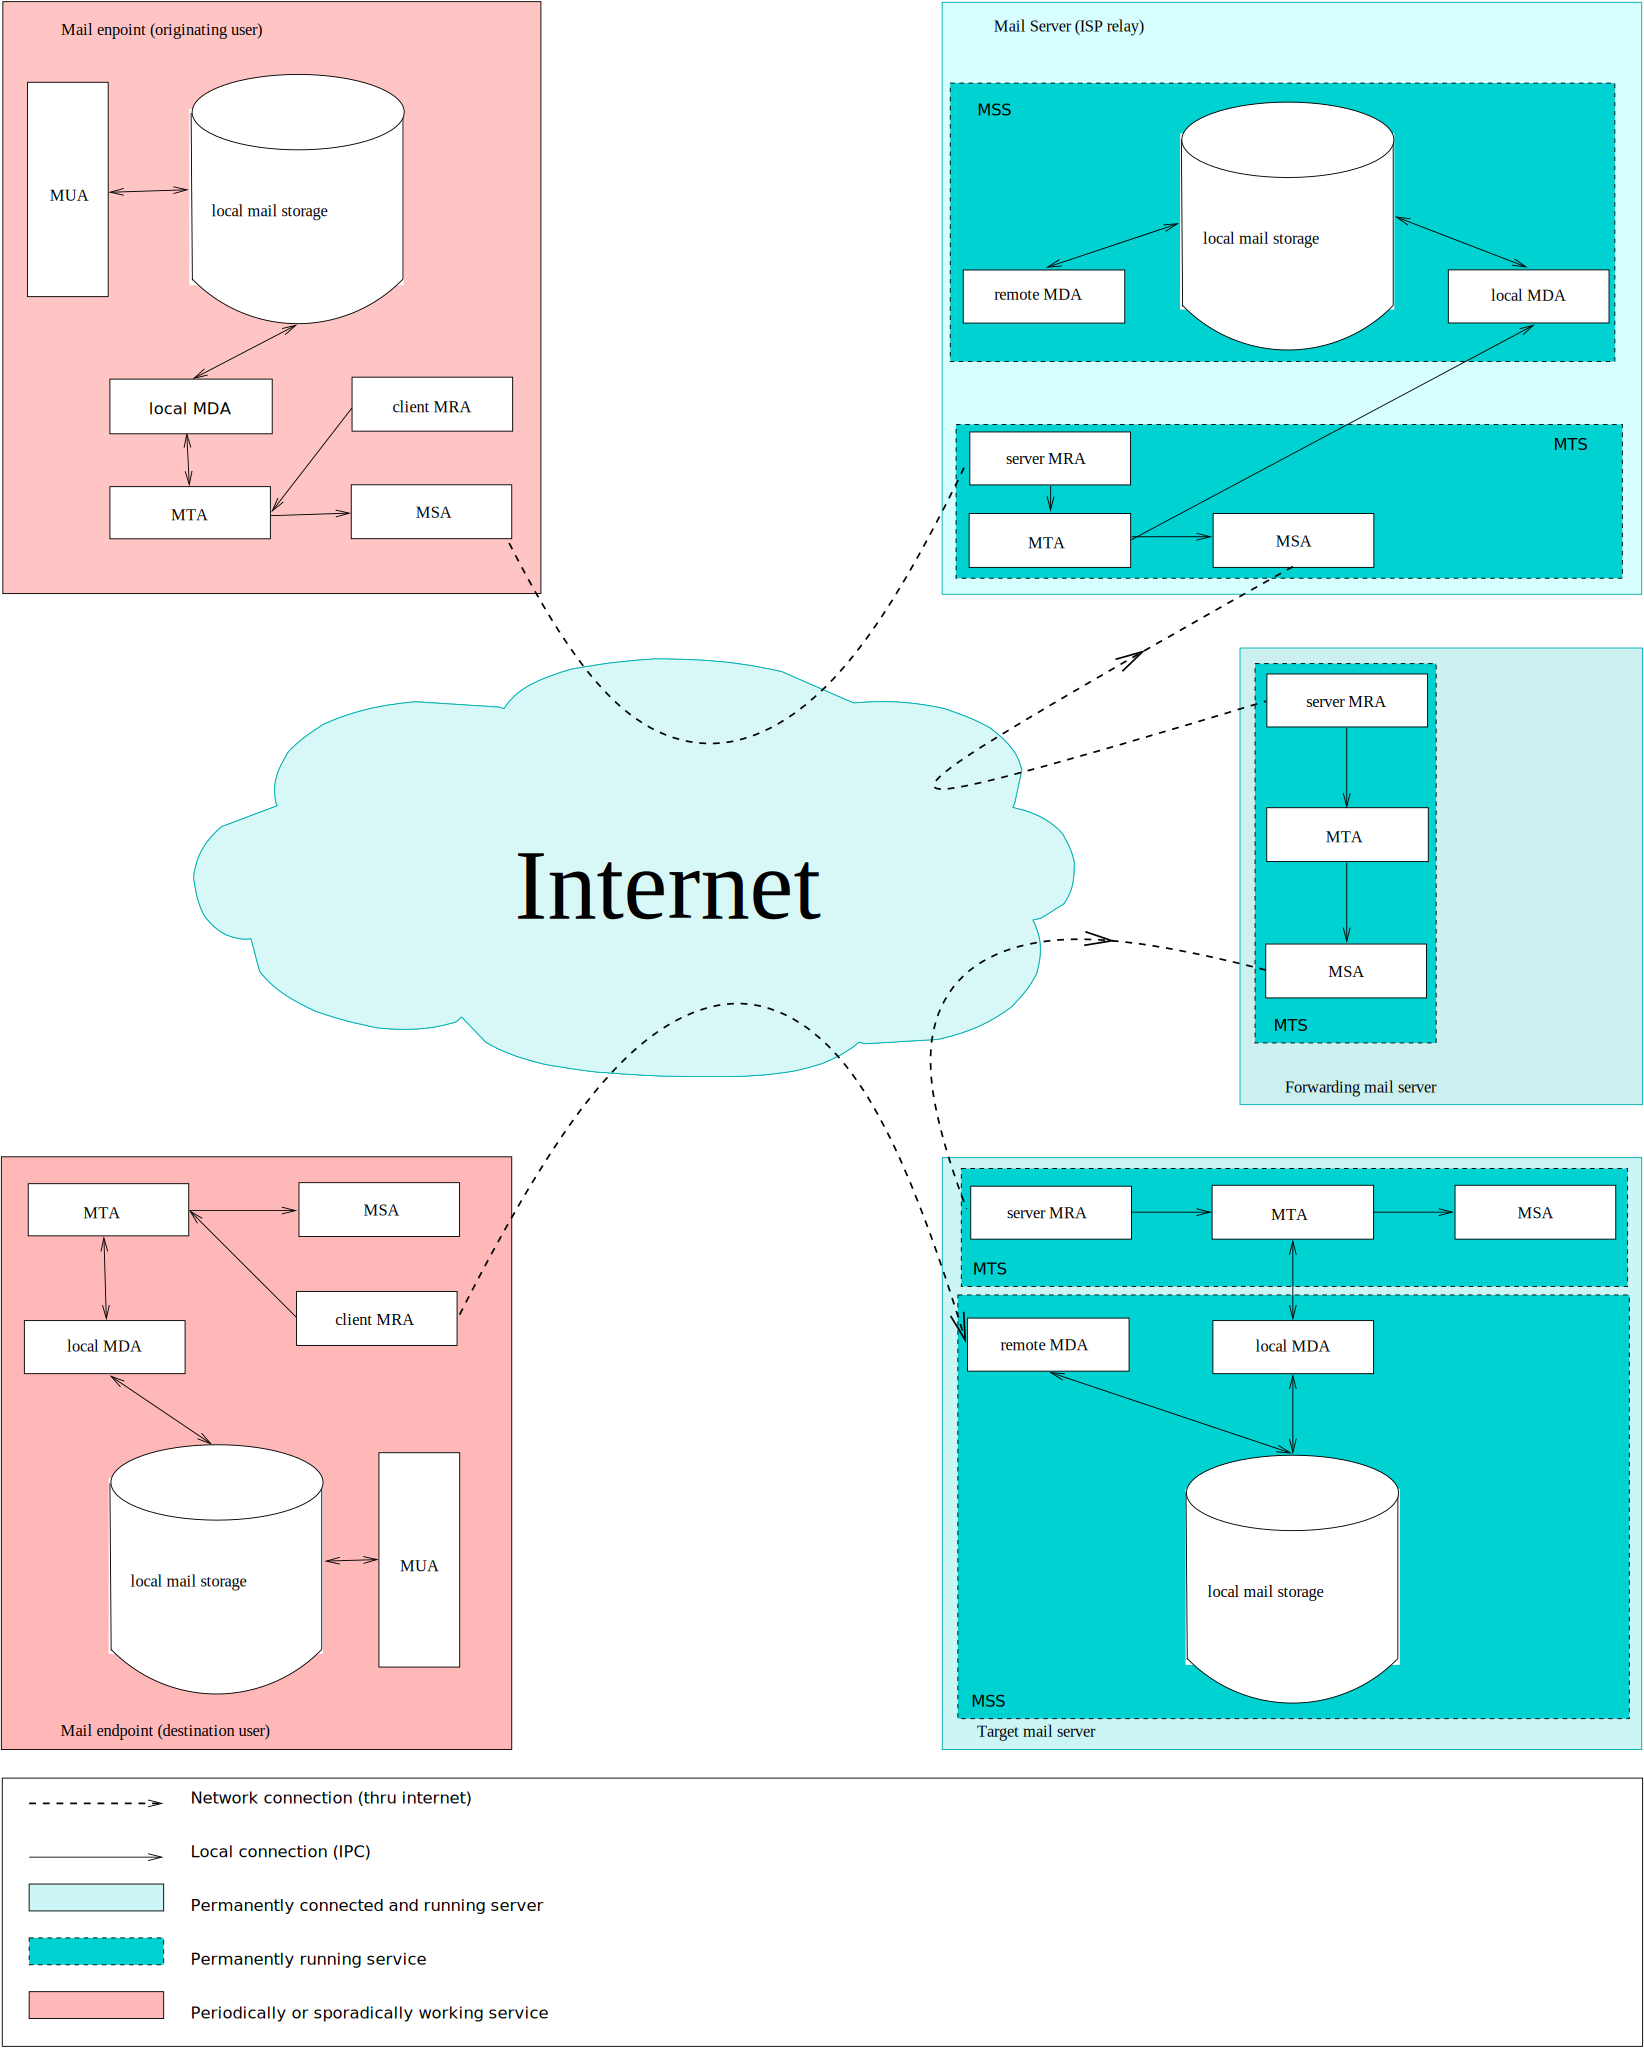
\includegraphics[width=\columnwidth]{inc/MailAgents1.pdf}
	\caption{Mail Agents}\label{fig:MailAgents}
\end{figure}

In the following paragraphs (for definitions), the term ``email'' is used synonymously to the term ``Message''.  ``Email'' has been chosen over ``messages'' because of its frequent use in standard documents.

Emails are typically initiated by a Mail User Agent (\defref{MUA}). An MUA accesses local email storage, which may be the server storage or a local copy. The local copy may be a cache only copy, the only existing storage (when emails are fetched and deleted from the server after retrieval), or a collected representation of multiple server storages (cache or authoritative).

Besides the MUA, the only other component accessing local email storage is the Mail Delivery Agent (\defref{MDA}). An MDA is responsible for storing and fetching emails from the local mail storage. Emails destined for other accounts than the current one are forwarded to the MTA. Emails destined to a User are persistently stored in the local email storage. It is essential to understand that email storage does not necessarily reflect a single mailbox. It may as well represent multiple mailboxes (e.g., a rich client-serving multiple IMAP accounts) or a combined view of multiple accounts (e.g., a rich client collecting mail from multiple \defref{POP} accounts). In the case of a rich client, the local MDA is part of the software provided by the user agent. In the case of an email server, the local MDA is part of the local email store (not necessarily of the mail transport service).

On the server-side, there are usually two components (services) at work. A ``Mail Transport Service'' (\defref{MTS}) responsible for mail transfers and a ``Mail Storage System'' which offers the possibility to store received Mails in a local, persistent store.\par

An MTS generally consists out of three parts. For incoming connects, there is a daemon called Mail Receiving Agent (\defref{Server MRA}) is typically a \defref{SMTP} listening daemon. A Mail Transfer Agent (\defref{MTA}) which is responsible for routing, forwarding, and rewriting emails. Moreover, a Mail Sending Agent (\defref{MSA}) which is responsible for transmitting emails reliably to another Server MRA (usually sent via \defref{SMTP}).\par

An MSS consists of local storage and delivery agents which do offer uniform interfaces to access the local store. They do also deal with replication issues, and grant should take care of the atomicity of transactions committed to the storage. Typically there are two different kinds of \defref{MDA}s. \defref{Local MDA}s offer possibilities to access the store via efficient (non-network based) mechanisms (e.g., IPC or named sockets). This is usually done with a stripped-down protocol (e.g., \defref{LMTP}). For remote agents there a publicly -- network-based -- agent available. Common Protocols for this \defref{Remote MDA}\ include \defref{POP}, \defref{IMAP}, or \defref{MS-OXCMAPIHTTP}.\par

Mail endpoints consist typically of the following components:
\begin{itemize}
	\item A Mail User agent (\defref{MUA})
	\item A Local Mail storage (\defref{MUA})
	\item A Local Mail Delivery Agent (\defref{Local MDA})
	\item A Mail Transfer Agent (\defref{MTA})
	\item A Mail Sending Agent (\defref{MSA})
	\item A Mail Receiving Agent (\defref{MRA})
\end{itemize}

Only two of these components do have external interfaces. These are \defref{MSA} and \defref{MRA}. \defref{MSA} usually uses \defref{SMTP} as transport protocol. When doing so, there are a couple of specialties. 
\begin{itemize}
	\item Port number is 587 (specified in \cite{RFC4409}).\\
	Although port numbers 25 and 465 are valid and do usually have the same capabilities, they are for mail routing between servers only. Mail endpoints should no longer use them.
	\item Connections are authenticated.\\
	Unlike a normal server-to-server (relay or final delivery) SMTP connections on port 25, clients should always be authenticated of some sort. This may be based on data provided by the user (e.g., username/password or certificate) or data identifying the sending system (e.g., IP address)\cite{RFC4409}. Failure in doing authentication may result in this port being misused as a sender for \defref{UBM}.
\end{itemize}

Mail User Agents (MUA) are the terminal endpoint of email delivery. Mail user agents may be implemented as fat clients on a desktop or mobile system or as an interface over a different generic protocol such as HTTP (Web Clients). 

Server located clients are a special breed of fat clients. These clients share the properties of fat clients except for the fact that they do not connect to the server. The client application itself has to be run on the server where the mail storage persists. This makes delivery and communication with the server different. Instead of interfacing with an MSA and a client MDA, they may directly access the local mail storage on the server. On these systems, the local mail storage may be implemented as a database in a user-specific directory structure.

\subsubsection{Fat clients}
The majority of mail clients are fat clients. These clients score over the more centralistic organized web clients in the way that they may offer mail availability even if an Internet connection is not available (through client-specific local mail storage). They furthermore provide the possibility to collect emails from multiple sources and store them in the local storage. Unlike Mail servers, clients are assumed to be not always online. They may be offline most of the time. To guarantee the availability of a particular email address, a responsible mail server for a specific address collects all emails (the \defref{MSS} does this) and provides a consolidated view onto the database when a client connects through a local or remote MDA.

As these clients vary heavily, it is mandatory for the MDA that they are well specified. Lack of doing so would result in massive interoperability problems. Most commonly the Protocols \defref{IMAP}, \defref{POP} and \defref{EWS} are being used these days. For email delivery, the SMTP protocol is used. 

Fat clients are commonly used on mobile devices. According to  \cite{clientDistribution} in Aug 2012 the most typical fat email client was Apple Mail client on iOS devices ($35.6\%$), followed by Outlook ($20.14\%$), and Apple Mail ($11\%$). \citetitle{clientDistribution2}\cite{clientDistribution2} as a more recent source lists in February 2014 iOS devices with $37\%$, followed by Outlook ($13\%$), and  Google Android ($9\%$).

\subsubsection{Server located clients}
Server located clients build an absolute minority. This kind of clients was common in the days of centralized hosts. An example for a Server Located Client is the Unix command ``mail''. This client reads email storage from a file in the users home directory.

\subsubsection{Web clients}
Web clients are these days a common alternative to fat clients. Most big provider companies use their proprietary web client. According to \cite{clientDistribution2} the most common web clients are "`Gmail"', "`Outlook.com"', and "`Yahoo! Mail"'. All these Interfaces do not offer a kind of public plug-in interface. However,  they do offer IMAP-interfaces. This important for a future generalistic approach to the problem.

\section{S/MIME (1996)}
S/MIME is an extension to the MIME standard. The MIME standard allows in simple text-oriented mails an alternate representation of the same content (e.g., as text and as HTML), or it allows to split a message into multiple parts that may be encoded. It is important to note that MIME encoding is only effective in the body part of a mail.

S/MIME, as described in \cite{RFC3851}, extends this standard with the possibility to encrypt mail content or to sign it. Practically this is achieved by either putting the encrypted part or the signature into an attachment. It is essential to know that this method leaks significant pieces of the data.

As the mail travels directly from sender to recipient, both involved parties are revealed. Neither message subject nor message size or frequency is hidden. This method does offer limited protection when assuming an adversary with interest in the message content only. It does not protect from the kind of adversary in our case. 

The trust model is based on a centralistic approach involving generally trusted root certification authorities.

\section{Pretty Good Privacy (1996)}
Exactly as S/MIME PGP\cite{rfc4880} builds upon the base of MIME. Although the trust model in PGP is peer-based. The encryption technology does not significantly differ (as seen from the security model).

Like S/MIME, PGP does not offer anonymity. Sender and endpoints are known to all routing nodes. Depending on the version of PGP, some meta-information or parts of the message content such as subject line, the real name of the sender and receiver, message size is leaked.

A good thing to learn from PGP is that peer-based approaches are offering limited possibilities for trust. The trust in PGP is based on the peer review of users. This peer review may give an idea of how well verified the key of a user is.


% ********************************************************************************************************
% *** Decisions and Research
% ********************************************************************************************************
\part{Substancial Decisions and Research Related to MessageVortex}
\fxwarning{complete section}

MessageVortex is a protocol piggybacking common transport protocols somehow similar as S/MIME\cite{RFC2015} or PGP\cite{PGP} which are common transport protocols such as SMTP. 


\fxwarning{complete intro to the MessageVortex model}

\chapter{Threat Model}
We refer to jurisdiction as a geographical area where a set of legal rules created by a single actor or a group of actors apply, which contains executive capabilities (e.g., police, army, or secret service) to enforce this set of legal rules.

We assume for our protocol that adversaries are state-sponsored actors or players of large organizations. These actors have high funding and expected to have elaborated capabilities themselves or within reach of the sponsor. Actors may join forces with other actors as allies. However, achieving more than 50\% on a world scale is excluded from our model. We always assume one or more actors with disjoint interests covering half of the network or more. 

We assume the following goals for an adversary:
\begin{itemize}
	\item An adversary may want to disrupt non-authorized communication.
	\item An adversary may want to read any information passing through portions of the Internet.
	\item An adversary may want to build and conserve information about individuals or groups of individuals of any aspect of their life. 
\end{itemize}

To achieve these goals, we assume the following properties of our adversary:
\begin{itemize}
	\item An adversary has elaborated technical know-how to attack any infrastructure. This attack may cover any attack favoring his goals, starting with exploiting weaknesses of popular software (e.g., buffer overflows or zero-day exploits) down to simple or elaborated (D)DoS attacks.
	\item An adversary may monitor traffic at any point in public networks within a jurisdiction.
	\item An adversary may modify routing information within a jurisdiction freely.
	\item An adversary may freely modify even cryptographically weak secured data where a single or a limited number of entities grant proof of authenticity or privacy.
	\item An adversary may inject or modify any data on the network of a jurisdiction.
	\item An adversary may create their nodes in a network. He may furthermore monitor their behavior and data flow without limitation.
	\item An adversary may force a limited number of other non-allied nodes to expose their data to him. For this assumption, we explicitly excluded actors with disjoint interests.
	\item An adversary may have similar access to resources as within its jurisdiction in a limited number of other jurisdictions.
\end{itemize}

we may furthermore subdivide the adversaries into the following sub-classes:
\begin{itemize}
	\item A censoring adversary\\
	The primary goal of this adversary is censoring messages and opinions, not within his interests. He does this, regardless of whether the activities of censorship may be observed or not. Therefore, this adversary does not cloak its activities and typically bans censorship circumventing activities as illegal.
	\item An observing adversary\\
	This adversary behaves like a traditional spy. He collects and classifies information while hiding its activities. Unlike within reach of a censoring adversary, in this case, typically, no restrictions apply to the use of anonymization technology.
\end{itemize}

\chapter{Protocol Outline}
\fxwarning{complete section}
\chapter{Key Concepts}
\fxwarning{complete section}
\section{Nodes}
\fxwarning{complete section}
\section{Protocol Layers}
\fxwarning{complete section}
\section{Vortex Messages}
\fxwarning{complete section}
\section{Workspaces}
\fxwarning{complete section}
\section{Ephemeral Identities}
\fxwarning{complete section}
\section{Routing Operations}
\fxwarning{complete section}
\section{Routing}
\fxwarning{complete section}



\chapter{Identification of Possible Attack Schemes and Mitigation}
\fxwarning{complete section}
\section{Static Attacks}
\fxwarning{complete section}
\subsection{Bugging and Tagging Attacks}
\fxwarning{complete section}
\subsection{Information Leaking related to Information Available to Routing Nodes}
\fxwarning{complete section}
\subsection{Identification of involved Nodes}
\fxwarning{complete section}
\subsection{Identification of MessageVortex Traffic}
\fxwarning{complete section}
\section{Dynamic Attacks}
\fxwarning{complete section}
\subsection{Attacks against the vortex system itself}
%\subsubsection{DoS Attacks against the Transport System}
%\subsubsection{DoS by Traffic Replay}
%\subsubsection{DoS by Traffic generation}
\subsection{Attacking a single ephemeral Identity of a MessageVortex Node}
\fxwarning{complete section}
%\subsubsection{Denial of Service by Exhausting Quotas or Limits}
\subsection{Attacking Sending and Receiving Identities of the MessageVortex System}
\fxwarning{complete section}
%\subsubsection{Traffic Highlighting or Traffic Analysis}
\subsection{Recovery of Previously Carried Out Operations}
\fxwarning{complete section}

\chapter{Censorship Circumvention}
\fxwarning{complete section}
\section{Technical Forms of Censorship}
\fxwarning{complete section}
\section{Zero Trust}
\fxwarning{complete section}

\chapter{Message Blending}
\fxwarning{complete section}
\section{Plain Blending}
\fxwarning{complete section}
\section{F5 Blending}
\fxwarning{complete section}

\chapter{Message Structure}
\fxwarning{complete section}
\section{Identification of a Message}
\fxwarning{complete section}
\section{Message Structure Related to Censorship Circumvention}
\fxwarning{complete section}
\section{Message Structure Related to Information Leaking}
\fxwarning{complete section}

\chapter{Routing}
\fxwarning{complete section}
\section{Algorithms Suitable for Achieving Anonymity}
\fxwarning{complete section}
\section{Possibilities of Routing Diagnosis and Reputation Building}
\fxwarning{complete section}
\section{Possibilities of Redundancies}
\fxwarning{complete section}

\chapter{Protocol Bootstrapping}
\fxwarning{complete section}
\section{Key Distribution for Endpoints}
\fxwarning{complete section}
\section{Key Aquisition for Routing Nodes}
\fxwarning{complete section}


\part{Analysis of MessageVortex}
\fxwarning{complete section}
\chapter{Analysis of the effectiveness of Attack Schemes}
\fxwarning{complete section}
\chapter{Analysis of the Degree of Anonymization in Comparison to other Systems}
\fxwarning{complete section}

\part{Discussion on Results}
\fxwarning{complete section}

%!TeX program=pdflatex
%!TeX encoding=utf8
%!TeX spellcheck = en_GB
%!TeX root = mailvortex_new.tex

\part{Results}
To verify the hypothesis made in this paper, and to analyse properties of the protocol in a real world scenario a library was implemented in Java which was capable of handling all message packets and the routing stack as a whole. The following paragraphs describe the protocol developed in general as a generic approach. Appendix \ref{app:asnone} gives the full ASN.1 representation of the protocol. 

It is important to notice that ASN.1 has no mean to express encrypted structures. Due to this fact we defined all encrypted fields as \verb|OCTET STRING|. The protocol offers according to the ASN.1 the possibility to store onionized information in an unencrypted form. This is meant for debuing purposes. At no point this should be used in a production environment.

The protocol described in the next chapter is independent from routing. At the moment capabilities include SMTP and XMPP. The protocol may be extended by adding new transport layer capabilities and their addressing schemes.

\chapter{MessageVortex - Transport Independent Messaging anonymous to \nth{3} Parties}
This approach is different from all approaches discussed previously. Unlike them we put complete distrust into the infrastructure being used. Furthermore we do not rely on a custom server infrastructure in the internet. Instead we take advantage of the availability of internet connected devices such as internet connected mobile phones, tablets, or even commonly available SoC such as RaspberryPi or similar. It is still very hard to maintain a server in the internet and considering the vastly growing amount of automated attack carried out against internet connected servers it is not advisable or realistic to assume that a future user of this system owns either a server or connects to a service which is offering explicitly anonymizing services. These infrastructures would be suspectible to monitoring or even banning. Instead we take a different approach.

We use common messaging protocols as transport layers and connect to them using the respective client protocols. The actual mixes are operated by the users on their ``always connected'' devices. It goes without saying that such a system is far less reliable than a traditionally run server as this hardware is typically cheap and normally connected to the internet using a bandwidth shared media.

The basic idea is that a client generates all traffic (including decoy or dummy traffic) by itself. It defines the routes a message takes through the mixes and decides which targets are receiving dummy traffic at the same time. In such a system even when possessing all the nodes routing the traffic (without the endpoints) an anonymity set of $k$ (whereas the size of $k$ is defined by the sender) is guaranteed.

As decoy traffic is generated with the same operations as the true content is split it is impossible for an adverser running a node to determine wether he is generating noise or actually processing the true message.

\fxfatal{add a lot more text here}
\begin{figure}[h]
	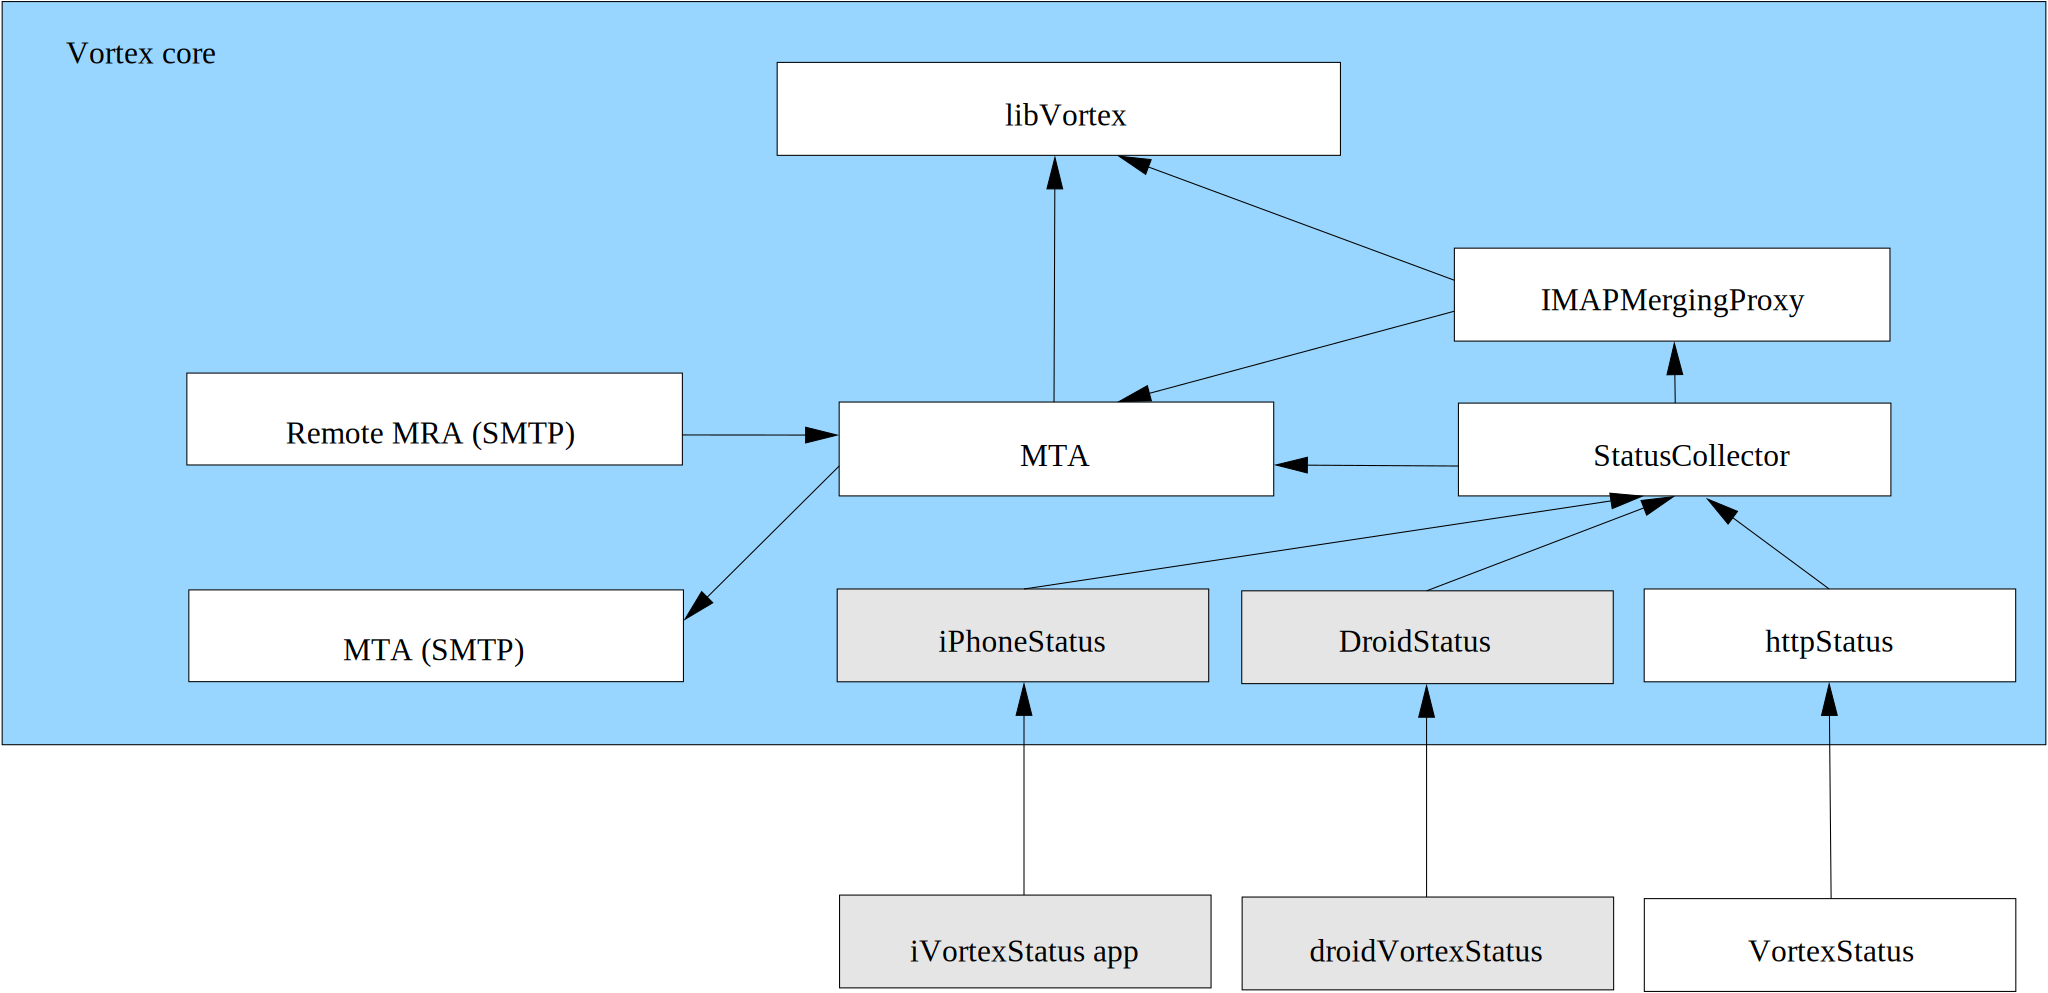
\includegraphics[width=\columnwidth]{inc/VortexModules.pdf}
	\caption{Overview of the Vortex modules}
	\label{fig:vortexModules}
\end{figure}

\section{Protocol Description}
\section{Accounting}
\section{Message Flows}

\section{Considerations for Building Messages}
In a worst case scenario we assume that an adverser is controlling most of the network utilized for anonymisation. While this is not nessessarily a problem (as pointed out earlier) it allows an adverser to track a message while agents are being used under his control. So for simplicity and as a worst case assumption we always assume that an adverser has perfect knowledge of an associated message flow. This is however a worst case scenario. One missing agent disconnects the whole chain and as messages are not traceable in size.

\subsection{Ephemeral identities}
\fxfatal{expiring ephemeral identities shold not only be replaced after their expiration but anytime during the livetime}
\subsection{Timing of messages}
\fxfatal{add content here}

\subsection{Building Diagnostic Paths}
\fxfatal{add content here}

\subsubsection{Implicit Diagnostic}
\fxfatal{Add comments about messages splitting and returning to sender}

\subsubsection{Automatic Explicit Diagnostic}
\fxfatal{Add comments about error and diagnosis messages officially spliting of messages}

\subsubsection{On-Demand Explicit Diagnostic}
\fxfatal{Add comments about normal, error, and diagnosis messages beeing picked up by a routing block}

\section{Considerations for Routing Messages}
\subsection{Time of sending}
Messages should always be sent timewise nearby other messages. This means that the best moment for sending a message in a ready queue is at a time when sending of other messages is due. However no optimisation should be done to send as many messages as possible at the same time. this would lead to a forseeable behaviour of the routing layer and thus to misusable behaviour.



\section{Real World Considerations}
This approach is heavily dependent of the transport protocol and builds on top a new obfuscating/routing layer. For this system to become a real peer-to-peer approach some additional quirks are required. A message-Vortex-Account needs always an active routing handler. This routing handler may be introduced by new server capabilities or by having a device handling the routing from the client side. For this reason we built a RaspberryPi appliance capable of connecting to one (or more) accounts fetching incomming mails, analysing them and reroute them if necessary. Although the system is designed to be run on a RaspberryPi the software might be installed to any Java capable client. The RaspberryPi is just an affordable lightweight device which offers all required capabilities.

\chapter{Security Analysis}
\fxfatal{add content here}

\chapter{Additional Considerations}
\fxfatal{add content here}

\section{Storage of Messages and queues}
The storage of messages sent though MessageVortex should be handled with great care. It seems on the first sight a good idea to merge all messages in a globally available storage such as the mail account of the receiving entity. However -- In doing so we would discover the message content to the providing party of a mail account. Since we handled the message with great care and tremendous costs up until this point it would be careless doing so. 

Storing them in a localized and receiving entity controlled storage is definitely a good idea but leaves security considerations like a backup possibly to an end user. This might be better but in effect a questionable decision. There is however a third option. By leaving the message unhandled on the last entity of the MessageVortex chain we may safely backup the data without disclosing the message content. Merging the content then dynamically through a specialized proxy would allow the user tu have a unified view on his without compromising the security.

\fxfatal{implemented in prototype?}

\section{Economy of transfer}
\fxfatal{Write something about wasting bandwidth}
%!TeX program=pdflatex
%!TeX encoding=utf8
%!TeX spellcheck = en_US
%!TeX root = ../../messageVortex.tex

\part{Discussion \label{sec:discussion}}

In the following chapters, we analyze the protocol thoroughly for fitness of purpose. 

We first apply a statical analysis of the protocol to identify all pieces of information leaked at all levels.

Then we apply a dynamic analysis of the protocol to identify all meta pieces of information leaked during transmission of the protocol such as timing or context between messages.

We distinguish between passive and active adversaries. Passive adversaries follow the MessageVortex protocol, have unlimited observation capabilities on the network up to layer 4 of the ISO/OSI protocol, and do have unlimited observation capabilities on the transporting layer of MessageVortex. Active adversaries share the capabilities of passive adversaries, but do not follow the MessageVortex protocol. Both adversaries try to obtain valuable information (e.g., message content, metadata such as the communicating peers or message frequencies). For a more precise model refer to \ref{sec:adversary}.

We then sum up the achieved goals by looking at well-known attacks and analyze the effectiveness of them to analyze the protocol.

At the very end of this chapter, we identify the gaps uncovered by this work.

\chapter{Static analysis}
In this section, we analyze the protocol statically. Looking at a full message, we get the protocol outline as shown in \eqref{eq:vortexMessage} on page~\pageref{eq:vortexMessage}.

\begin{figure*}[!h]
	\begin{align}
	VortexMessage                = &\langle \mathbf{MP}^{K^{-1}_{hostN}}, \langle\mathbf{PAD}, \mathbf{CP}^{K^{-1}_{hostN}}, \mathbf{H}^{K_{senderN}}, E^{K^{-1}_{senderN}}\left(H\left(\mathbf{HEADER}\right)\right)  \nonumber \\
	& \left[\mathbf{R}^{K_{senderN}}\right], \left[\mathbf{PL}\right]*\rangle^{K_{peerN}} \rangle\label{eq:vortexMessage}\\ 
	\mathbf{MP}^{K^{-1}_{hostN}}  = &E^{K^{-1}_{hostN}}\left(\mathbf{PREFIX}\langle K_{peerN}\rangle \right)\\ 
	\mathbf{PAD}                 = &\langle \text{32 padding bytes from payload} \rangle\\ 
	\mathbf{CP}^{K^{-1}_{hostN}} = &E^{K^{-1}_{hostN}}\left(\mathbf{CPREFIX}\langle K_{senderN}\rangle \right)\\ 
	\mathbf{H}^{K_{senderN}}     = &E^{K_{senderN}}\left(\mathbf{HEADER}\right)\\  
	\mathbf{HEADER}              = &\langle K^{1}_{senderN}, serial, maxReplays, validity, [requests, requestRoutingBlock],\nonumber\\ 
	& [puzzleIdentifier, proofOfWork] \rangle \\  
	\mathbf{R}^{K_{senderN}}     = & E^{K_{senderN}}\left(\mathbf{ROUTING}\right)\\ 
	\mathbf{ROUTING}             = & \langle [ \mathbf{ROUTINGCOMBO} ] *, forwardSecret, replyBlock \rangle\\  
	\mathbf{ROUTINGCOMBO}        = & \langle processIntervall, K_{peerN+1}, recipient, \mathbf{nextCP}, \mathbf{nextMP}, \nonumber \\
	& \mathbf{nextHEADER}, \mathbf{nextROUTING}, assemblyInstructions, id \rangle\\
	\mathbf{PL}                  = &\langle \text{payload octets} \rangle *\\ 
	\end{align}
	\captionsetup{labelformat=empty}
	\caption{Detailed representation of a VortexMessage}
\end{figure*}

\section{Transport and Blending Layer}

\subsection{Analysis of Plain Embedding}
It is very obvoious why a file treated with plain embedding is easily identifiable as a broken or tampered file. While the file is still parseable, its content is no longer sensible to a human and thus at least suspect. 

We wanted to know if there is an easy method to detect the modifications of such a file. While most of the analysis methode require processing of large data sets we tried to find obvious, non-calcualtion-intense test methods which were generic. We did not take any content based characteristics such as ``outline of an image'' or ``resulting spectrum of a soundfile'' in account. As our embedding is generic, we searched for a similar detection method.

A property of encrypted cipher text is the high entropy. We therefore used the calculation of the Shannon entropy in bytes as a property and tried to show the shift of entropy within the files. This detection method depended very much on the type of file used for embedding. It showed an expected behavior, that file types having in the expected area a similar entropy were not detectable by this method. However, the following file types were identified to be unsuitable for plain blending due to their entropy structure.

We analyzed the files by calculating the entropy of blocks 256 bytes and did this with a sliding window over a randomly collected set of images (e.g., the topmost 100 entries of a file type after searching for ``mouse'', ``cat'', ``camel'', or ``dog''). We did intentionally not filter or eliminate images. The finds were very surprising. We were able to identify tell file types apart, were able to identify files with thumbnails or an interlaced structure. We even identified certain specific pattern regarding the producer type of an image (e.g., we could differentiate between images scanned and images taken by a camera). It was not so much surprising that we were able to identify these features, but the fact that we could see them in entropy data.

\begin{figure*}[ht]
	\includegraphics[width=\textwidth]{inc/statanalysis_graph}
	\caption{distribution analysis of different common graphics formats}
	\label{fig:statGraph}
\end{figure*}

We then carried out an analysis identifying the typical entropy and the inner structures. The graphs in \ref{fig:statGraph} show a typical analysis. In that case we looked at 100 images of each type. We graphed and analyzed their entropy and tested for suitability of a plain embedding. Table \ref{tab:fileEntropy} lists the average entropy of analyzed file types and makes remarks about the suitability for plain embedding. In practice we found that most suitable file formats have an entropy of $\approx 7.2$ and an interquartile range (IQR) of 0.5 or less. Furthermore, files should have a big, uniformous, non structured range containing this characteristics so that they have a uniformous suitable space for embedding.

\begin{table*}[h]
	\centering\tiny
	\begin{tabular}{|l|l|l|l|}\hline
		\diaghead{\theadfont Type Criteria}{Type}{Criteria} & \thead{Avg. Entropy} 	& \thead{IQR} & \thead{Remarks}\\\hline
		JPG	   & 7.008  & 0.097  & -- \\              
		PNG	   & 7.116  & 0.086  & -- \\              
		GIF	   & 6.978  & 0.194  & -- \\              
		BMP	   & 2.997  & 4.964  & not suitable \\              
		PDF	   & 		&        & Hard to embed due to a very complex inner structure \\\hline              
		MP3	   & 7.076  & 0.091  & -- \\              
		wav	   & 		&        & -- \\              
		ogg	   & 7.104  & 0.093  & relatively easy to embedd. Hard not to break the structure. \\\hline              
		mpg4   & 		&        & good to embedd. Steganography could be applied here easily too. \\\hline              
		zip    & 		&        & easy to embedd when using ``password protected''  archives \\\hline              
	\end{tabular}	
	\caption{comparison of protocols in terms of the suitability criteria as transport layer}
	\label{tab:fileEntropy}
\end{table*}

\fxwarning{Fill entropy table with values}

When blending into images, BMP showed a strongly varying entropy within a file. A sampling of ten blocks at random position resulted already in a detection with a failure rate below 5\%. PNG and JPG files showed to be very robust within the sample. We did not succeed in identifying the MessageVortex blending content absed on entropy values. GIF images showed to be unsuitable. Archive formats such as zip files were extremely robust. We were able to embed into zip and marking it (generically) as a password encrypted file. This embedding was truly undetectable.


\subsection{Identifying a Vortex Message Endpoint}
Depending on the blending method, single messages might be identified as long as they are detectable. Detectability depends on various factors such as:

\begin{itemize}
	\item Broken internal file structure (due to plain blending)
	\item Uncommon high entropy in a structureless file
	\item Unrelated message flow (see \cite{oakland2013-parrot})
	\item Non-human behaviour on the transport layer (e.g., message traffic 24x7)
\end{itemize}

If an endpoint is successfully identified, then all directly related endpoints of the same protocol may be identified as well by following the message flow. This does however not enable an adversary to inject messages as the host key is not leaked. 

Assuming a global observer as an adversary and unencrypted traffic, he might discover the originating routing layer and thus identify it as Vortex node by following traces of the transport layer. In most protocols, however, this address is spoofable and not a reliable source for the originating account.

\section{Senders routing layer}
A sender may have some knowledge about the Routing block size and may, therefore, guess the complexity of the routing path. He is, however, unable to gain any additional information such as time of travel or number of hops until the target.

\section{Intermediate node routing layer}
An intermediate node does know all the operations applied and the immediate next hop. It does learn the routing addresses of the immediately following endpoints but is unable to use these endpoints. This is because he has no mean to get the host key required to communicate.

If a routing block is repeated, a router may identify the routing block as repetition due to the serial number of the replay protection and give a rough estimate about the message size by comparing the payload chunks. This estimate is however very rough as it is bounded by the block size of the symmetrically applied encryption.

\chapter{Dynamic analysis}
In the dynamic analysis, we reach out to an active adversary. An active adversary modifies traffic in a non-protocol conformant way, or missuses available or obtained information to disrupt messages, nodes, or the system as a whole.

\section{Attacks against the vortex system itself}
An active adversary may attack the transport layer. Most of the transport layers are not able to react upon message flooding. Therefore, it is easy to attack a transport layer with a flooding attack, such as a distributed denial of service (DDoS) attack. Due to the nature of the protocol, we are unable to apply for additional protection on the transport layer or below. The Vortex Message format itself is however crafted in such a way that only minimal effort is sufficient to get the involved parties of a transmission. The Operations $ K_{msgN}=D^{K^{1}_{host}}\left(P\right)$ and $HEADER=D^{K_{msgN}}\left(H\right)$ are sufficient to identify message senders. Unknown Senders may be discarded without further processing. Known senders may be identified as legitimate and processed further. Known misbehaving identities and message duplicates may be discarded. 


\subsection{DoS Attacks against the System}
An active adversary may not follow the protocol and modify any parts of the message. The following paragraphs reflect different kinds of behavior and how they affect the messages and the system as a whole.

An adversary may not follow the blending specification. If he uses a specification which is less secure an independent third party observer may follow traffic. This is not sensible as such a node may send all the knowledge to such a collaborating node directly. In the case of a  target node not supporting the chosen blending method, the partial message path becomes interrupted. A possible redundancy in the path may recover the message from such a case.

\subsubsection{Traffic Replay}
Traffic replay is a common way to highlight traffic in many systems by replaying the same traffic and increase the signal to noise ratio of a system. 

Due to the replay protection of the vortex protocol, this is not possible. Any traffic generated by an attacking node is already known. Any subsequent messages of other nodes are only generated once even if a message is repeatedly received.

\subsection{Diagnosability of traffic}

\subsubsection{Hijacking of Header and Routing Blocks}
An attacker might try to recombine a header block of a third party with a routing block crafted to get workspace content of a different node. To protect against this scenario every routing block and its corresponding header block have a common value called forward secret. As the content of a hijacked header block is not known he is unable to guess the forward secret within the block.

It is not possible to brute-force the value, due to the replay protection. More precisely, the probability for hijacking a single identity block is $\frac{1}{2^{32}}$. If taking into account that a routing block may be replayed to the absolute maximum probability rises to $\frac{2^8-1}{2^{32}}\approx\frac{1}{2^{24}}$. Hijacking such a block allows onetime access to the working space and is visible to the owner due to the manipulated quotas. Failing of an attack will result in exhausting the ephemeral identities quotas, and a new unlinked ephemeral identity will be created. 


\subsubsection{Partial Implicit Routing Diagnosis}
We can create data which is routed back to or through the original sending node. This traffic is well defined and may be used to certify that the loop processing the message is working as expected. By combining the messages and sending intermediate results through multiple paths, it is even possible to extract the sub status of some loops and combine the result within transfer into a single message.

As a special case, implicit routing diagnostic may be used to diagnose the full route by taking specific excerpts from a message and routing them from the recipient back to the sender. 

\subsubsection{Partial Explicit Routing Diagnosis}
If a message fails to deliver according to implicitly routing diagnosis, additional messages may be sent to pick up the content of the workspace of ephemeral identities throughout the path. These messages are due to the only binding to the ephemeral identity not distinguishable from the original messages. Assuming that a node always behaves either according or not according to the rules of the system, a node may be identified.

\subsubsection{Denial of Service by Exhausting Quotas or Limits}
A malicious node may try to exhaust quotas or limits. As we do trust in sender and recipient, all other nodes do not know the forward secrets used in the message. The options for an adversary are then as follows:

\begin{itemize}
	\item Resend a MURB (with different content) as often as possible to exhaust message and transfer quota.
	\item Create intentionally huge, incorrect message content to exhaust transfer quota.
\end{itemize}

\subsubsection{Traffic Highlighting}
Traffic caused by a routing block may be observed by to a certain extent on a statistical base. A node may generate bad message content of exceptionally large or small nature this might potentially highlight messages involved in message routing using no split or relative split operations as well as addRedundancy operations.

\section{Achieved Anonymity and Flaws}
\subsection{Measuring Anonymity}
It is tough to measure anonymity as it involves many uncontrollable factors. We may, however, control the degree of anonymity according to the number of involved parties. Assuming a sender knows the complete message path including all operations carried out on any untrusted node a message travels through, the anonymity is maxed to the number of involved nodes $n$ excluding the sender nodes. This degree of $n-1$ may be further reduced if all well-known ``routing only'' or at least ``routing mostly'' nodes are reduced. Under these harsh assumptions, the set may be reduced to the potential set of ``well known'' recipients of a message.

We have to differentiate between several problems. An adversary has to identify the participants of an anonymity system. Then he has to identify members of a message or a communication anonymity set. Starting from there he has to identify message flows and detect senders and receivers of messages within an anonymity set (which is not doable in all cases). If any adversary achieves this, we have to consider the anonymity to be broken. Depending on the degree of anonymity required which is influenced by external factors the participation in any or a small enough set may be sufficient to suffer consequences.

\subsection{Attacking Routing Participants}
While very hard in our case as we do not have ``dedicated'' anonymization infrastructure, It might be possible to identify members of the routing network. This due to flaws in the blending layer. While it is possible to scare off or block members of a routing network. It is far harder in a network where the members are mobile. Any user may change at any time the identity including the endpoint without losing its known peers.

\subsection{Attacking Anonymity through Traffic Analysis}
As traffic and decoy traffic and decoy traffic are chosen by the creator of the routing block frequency patterns cannot be detected, unlike the router did create them. Same applies to message sizes and traffic hotspots. When reusing the same routing block eventually message sizes or general estimates such as ``bigger'' or ``smaller size'' can be made.

\subsection{Attacking Anonymity through Timing Analysis}
Timing is under full control of the routing block builder. No information can be derived from timing. This is even the case if a routing block is reused.

\subsection{Attacking Anonymity through Throughput Analysis}
Increasing the throughput to highlight a message channel is not possible since the replay protection will block such requests.

\subsection{Attacking Anonymity through Routing Block Analysis}
The routing block is cryptographically secure. The size of the routing block may leak an estimate about its inner complexity. It does not reveal any relevant pieces of information like remaining hops to the message end or target or similar.

\subsection{Attacking Anonymity through Header Analysis}
The header contains valuable data which is cryptographically secured and only visible to the next receiver. 

To an adversary not knowing the key, the size of the prefix block may leak the key size. The size of the header block itself may leak the presence of any optional blocks. Besides that, no other information is leaked to such an adversary.

To an adversary knowing the decryption key (evil routing node), the content of the header block is visible. This header block leaks all routing information for the respective node and thus the ephemeral identity. This block leaks some information of minimal value. It may leak the activity of an ephemeral identity including frequency. This activity is always matching the minimal activity of an endpoint identity. 

\subsection{Attacking Anonymity through Payload Analysis}
The payload itself does not leak any information about the message content. All content is cryptographically secured. Content may, however, leak the size of a key applied.

\subsection{Attacking Anonymity through Bugging}
Bugging is one of the most pressing problems. The protocol has been carefully crafted not to allow any bugging. The use of MIME messages in the final message, however, allows bugging of the message itself. A bugged message content may breach receiver anonymity to the sender of the message.

\subsection{Attacking Anonymity through Replay Analysis}
Due to the replay protection, no traffic may be generated or multiplied except for the traffic sent by the attacking node. As this information is already known to the node, there is no value in doing so. 

\chapter{Recommendations on Using the Vortex Protocol}
The following sections list recommendations using the VortexProtocol it is a summary of previous sections.

\section{Reuse of Routing blocks\label{sec:reuseRB}}
Routing blocks should not be reused. The reuse of a routing block may leak some limited information to an adversary node such as approximate message size or message frequency of an unknown tupel using this network.

\section{Use of Ephemeral Identities}
Ephemeral identities should be used for a minimal number of messages. Using multiple identities with overlapping lifespans is considered a good practice. Using different ephemeral identities for the same message is acceptable and may be a good practice as long as operations do not leak the linking between those two identities.

\section{Recommendations on Operations applied on Nodes}
All operations, carried out on a single node, have to be crafted in such a way that no information whether the operation is a decoy or a real message is leaked. Otherwise, it becomes possible to narrow down the message flow.

\section{Recommendations on Choosing involved Nodes}
Involved nodes should be trustworthy but not necessarily trusted. To avoid an adversary to control all nodes except for sender and receiver a message should always include a set of known recipients. It is regarded as a good practice to use a minimal fixed anonymity set of known recipients as routers. Doing so does not leak any information unless always the same pattern of operations is applied (see \ref{sec:reuseRB}).

\section{Message content}
Although it is possible to embed any content into a Vortex message great care should be taken as content may allow disclosing a readers identity or location. For this reason, only self-contained messages should be used (such as plain text messages).

\subsection{Splitting of message content}
Message content should be split and distributed among routing nodes. Splitting should however not be done excessively to avoid failure due to too many failing nodes. It furthermore makes diagnostics complicated. 

\section{Routing}

\subsection{Redundancy}
Redundancy is a valuable feature of the protocol. It allows unsuspicious decoy generation and to compensate message path disruption. A routing block should always be crafted in such a way that redundancy is aligned with the complexity of the routing block and the importance of a message.

\subsection{Operation Considerations}
Operations should be kept easy but at the same time guarantee anonymity. The following recommendations are kept to an absolute minimum in order not to create any identifiable behavior.

A payload block should always have a single representation only once when traveling through routing nodes. A recurring pattern would allow an evil router to identify and thus match an ephemeral identity of one router to an ephemeral identity of another router even if there are multiple routes in between. So, when applying encryption only operations between routing nodes, the encryption should be onionized. A clear onionizing routing pattern (only showing encryption steps on a single chunk) is OK. A pattern such as removing encryption and then reapply different encryption is not.

\subsection{Anonymity}
Anonymity is greatly dependent on the quality of the routing block and the chosen anonymity set for a single message and a communication tuple over time. 

\subsubsection{Size of the Anonymity Set}
The requirement for an anonymity set is dependent on jurisdictional restrictions. In some of the more restrictive countries, no one can be held guilty for an action which may not be credibly assigned to him alone. In other jurisdictions, it is possible to be held guilty for actions just because of an identified membership to a group. This makes it essential that message traffic and the crafting of the blending is under the sole control of the sender. He needs to create an anonymity-set sufficiently large and spanning enough jurisdictions to create sufficient anonymity for his situation.

\chapter{Missing gaps to be covered in future analysis}
The current blending layer is simple in its inner working. It creates context-less messages based on an easily recognizable scheme. An unsuspecting observer may have the impression that this is just a way of communicating but censor may by observing the message flow easily and conclude that these messages are not written by a human.

To be undetectable all work done by the blending layer has to be indistinguishable from regular human communication. This applies not only to the message steganographic embedding of the message but to the message content as well. This is very much similar to the problems of chatterbots these days. Assuming that a blending layer is only communicating with other nodes correctly embedding messages we have a chatterbot problem. It is reduced as the chatterbot must only reply credibly and undetectable to generated messages of other chatterbots. If assuming that a blending layer replies to any non-Vortex nodes the problem boils down to a Turing test as stated in \cite{turing1950computing}. As we safely may assume that an adversary has enormous but limited resources this blending is however sufficient if it is done ``good enough''. What criteria would apply here is a topic for further research. Applying any research to this topic would require to add a more precise adversary model.

The currently applied choice of transport layer protocol is a snapshot of current internet traffic. While done with great care it must be adapted to the changing communication habits of humanity. Identifying new or depreciated communication protocols and blending schemes would be another field of research.

A comprehensive survey of the newest trends and techniques in steganography is another topic to be covered. It would allow identifying new candidates of blending techniques.

Another problem is the software update. Where censorship applies to access to newer software is not or only with technical knowledge possible. To allow a user to update his software, an updating mechanism should be implemented allowing nodes to fetch verifiable software updates anonymously while not limiting the software to a single distribution.

Anonymity has effects on the behavior of humans. We have found that although there is some research in this field (such as \cite{postmes2001social}) evidence is very weak. Although the possibility for anonymity is undisputed among so-called free countries, the downsides (e.g., misuse for criminal acts) of anonymity are apparent. More research in this filed is required as well.




\backmatter
\pagenumbering{arabic}% resets `page` counter to 1
\renewcommand*{\thepage}{A\arabic{page}}
\appendix
\part{Appendix}
\makeatletter
\g@addto@macro\appendix{%
	\renewcommand*{\chapterformat}{%
		{\chapapp\nobreakspace\thechapter\autodot\enskip}%
	}
	\renewcommand*{\chaptermarkformat}{%
		{\chapapp\nobreakspace\thechapter\autodot\enskip}%
	}
	\let\oldaddcontentsline\addcontentsline
	\newcommand\hackedaddcontentsline[3]{\oldaddcontentsline{#1}{#2}{\chapapp\nobreakspace#3}}
	\let\oldchapter\chapter
	\renewcommand*\chapter[1]{%
		\let\addcontentsline\hackedaddcontentsline%
		\oldchapter{#1}%
		\let\addcontentsline\oldaddcontentsline%
	}
}
\makeatother
\onecolumn
%\chapter{The RFC draft document\label{app:rfcMessageVortexMain}}
%\includepdf[pages=-,frame=true,scale=0.5]{rfc/draft-gwerder-messagevortexmain-00.pdf}
\includepdf[pages=1,frame=true,scale=0.8,pagecommand=\chapter{The RFC draft document\label{app:rfcMessageVortexMain}}, offset=0 -1cm]{rfc/draft-gwerder-messagevortexmain-00.pdf}
\includepdf[pages=2-,frame=true,scale=0.8,pagecommand={}, offset=0 -1cm]{rfc/draft-gwerder-messagevortexmain-00.pdf}

\twocolumn
\chapter{Glossary}

\begin{entry}
  \mainentry{adverser}{FIXME}
\end{entry}

\begin{entry}
  \mainentry{Agent}{FIXME}
\end{entry}

\begin{entry}
  \mainentry{EWS}{FIXME}
\end{entry}

\begin{entry}
  \mainentry{IMAP}{IMAP (currently IMAPv4) is a typical protocol to be used between a \defref{Client MRA} and a \defref{Remote MDA}. It has been specified in its current version in \cite{RFC3501}. The protocol is capable of fully maintaining a server based message store. This includes the capability of adding, modifying and deleting messages and folders of a mailstore. It does not include however sening mails to other destinations outside the server based store.}
\end{entry}

\begin{entry}
	\mainentry{Item of Interest (IoI)}{FIXME}
\end{entry}

\begin{entry}
  \mainentry{LMTP}{FIXME}
\end{entry}

\begin{entry}
  \mainentry{Local Mail Store}{A Local Mail Store offers a persistent store on a local non volatile memory in which messages are beeing stored. A store may be flat or structured (eg. supports folders). A Local Mail Store may be an authoritative store for mails or a ``Cache Only'' copy. It is typically not a queue.}
\end{entry}

\begin{entry}
  \mainentry{mail server admin}{FIXME}
\end{entry}

\begin{entry}
  \mainentry{MDA}{An MDA provides an uniform access to a \defref{Local Mail Store}.}
  \subentry{Remote MDA}{A Remote MDA is typically supporting a specific access protocol to access the data stored within a \defref{Local Mail Store} .}
  \subentry{Local MDA}{A Local MDA is typically giving local applications access to a server store. This may be done thru an API, a named socket or similar mechanisms.}
\end{entry}

\begin{entry}
  \mainentry{MRA}{A Mail receiving Agent. This agent receives mails from a agent. Depending on the used protocol two subtypes of MRAs are available.}
  \subentry{Client MRA}{A client MRA picks up mails in the server mail storage from a remote MDA. Client MRAs usually connect thru a standard protocol which was designed for client access. Examples for such protocols are \defref{POP} or \defref{IMAP}}
  \subentry{Server MRA}{Unlike a Client MRA a server MRA listens passively for incomming connections and forwardes received Messages to a MTA for delivery and routing. A typical protocol supported by an Server MRA is \defref{SMTP}}
\end{entry}

\begin{entry}
  \mainentry{MS-OXMAPIHTTP}{FIXME}
\end{entry}

\begin{entry}
  \mainentry{MSA}{A Mail Sending Agent. This agent sends mails to a \defref{Server MRA}. }
\end{entry}

\begin{entry}
  \mainentry{MTA}{A Mail Transfer Agent. This transfer agent routes mails between other components. Typically  an MTA receives mails from an MRA and forwardes them to a MDA or MSA. The main task of a MTA is to provide reliable queues and solid track of all mails as long as they are not forwarded to another MTA or local storage.}
\end{entry}

\begin{entry}
  \mainentry{MTS}{A Mail Transfer Service. This is a set of agents which provide the functionallity tor send and receive Messages and forward them to a local or remote store.}
\end{entry}

\begin{entry}
  \mainentry{MSS}{A Mail Storage Service. This is a set of agents providing a reliable store for local mail accounts. It also provides Interfacing which enables clients to access the users mail.}
\end{entry}

\begin{entry}
  \mainentry{MUA}{A Mail User Agent. This user agent reads mails from a local storage and allows a user to read existing mails, create and modify mails.}
\end{entry}

\begin{entry}
  \mainentry{Privacy}{From the Oxford English Dictionary: ``
    \begin{enumerate}
      \item The state or condition of beeing withdrawn from the society of others, or from the public intrest; seclusion. The state or condition of beeing alone, undisturbed, or free from public attention, as a matter of choice or right; freedom from interference or intrusion.
      \item Private or retired place; private apartments; places of retreat.
      \item Absence or avoidance of publicity or display; a condition approaching to secrecy or concealment. Keeping of a secret.
      \item A private matter, a secret; private or personal matters or relations; The private parts.
      \item Intimacy, confidential relations.
      \item The state of being privy to some act.
    \end{enumerate}''\cite[FIXME]{OXFORD}\\
    In this work privacy is related to definition two. Mails should be able to be handled as a virtual private place where no one knows who is talking to whom and about what or how frequent (except for directly involved people).
  }
\end{entry}

\begin{entry}
  \mainentry{POP}{POP (currently in version 3) is a typical protocol to be used between a \defref{Client MRA} and a \defref{Remote MDA}. Unlike \defref{IMAP} it is not able to maintain a mail store. Its sole purpose is to fetch and delete mails in a server based store. Modifying Mails or even handling a complex folder structure is not doable with POP}
\end{entry}

\begin{entry}
  \mainentry{Service}{FIXME}
\end{entry}

\begin{entry}
  \mainentry{SMTP}{SMTP is the most commonly used protocol for sending mails across the internet. In its current version it has been specified in \cite{RFC5321}.}
\end{entry}

\begin{entry}
  \mainentry{Storage}{A store to keep data. It is assumed to be temporary or persistent in its nature.}
\end{entry}

\begin{entry}
  \mainentry{user}{FIXME}
\end{entry}

\begin{entry}
  \mainentry{UBE}{FIXME}
\end{entry}

\chapter{Bibliography}
{
  %\def\filespliter#1{\expandafter\intfilespliter#1\relax}
  %\def\intfilespliter#1 #2 #3\relax{ First: (#1), Second: (#2), Third: (#3) }
  \DeclareFieldFormat{file}{\StrGobbleLeft{#1}{1}[\wtcGwM]\StrGobbleRight{\wtcGwM}{4}[\filename] \IfFileExists{\filename}{\attachfile{\filename}}{FIXME missing document link}}
  \renewbibmacro{finentry}{\finentry\addspace \printfield{file}}
  \renewcommand*{\bibfont}{\small}
  \printbibliography[title={},heading=none]
}

% additional reference entries
\index{Mail transport|see {Message Transport}}

% add the index
\printindex

\begin{comment}
% just a trick to make TexNicCenter Bibliography working
\bibliography{messageVortex}
\bibliography{inc/bib/unclassified/Anonbib/anonbib}
\end{comment}



\begin{comment}
% Some Notes 
http://www.rfc-editor.org/pubprocess.html
RFC2223 Instructions to RFC Authors
RFC3979 BCP79 Intellectual Property Rights in IETF Technology
RFC5378 BCP78 Rights Contributors Provide to the IETF Trust


http://tex.stackexchange.com/questions/36307/formatting-back-references-in-bibliography
http://www.cs.columbia.edu/irt/software/l2x/ l2x -- conversion from LaTeX to other formats Version 1.13
http://ftp.gwdg.de/pub/ctan/support/l2x/
http://tools.ietf.org/tools/xml2rfc2

http://www.zisc.ethz.ch/events/2003-2011/ISC2006Slides/FederrathZISCTalk.pdf

Professorliste
Dr. Christoph Sprenger (Part I)
-Prof. David Basin
Gregory Demay
Peter Gazi
Dr. Srdjan Marinovic
Dr. Sasa Radomirovic
Dr. Ralf Sasse

T. Hoefler
A. Perrig 
-Dr. Jan Camenisch (Keine Berechtigung)

-Srdjan Capkun (Keine Kapazität)
-David Basin  (Keine Kapazität)
\end{comment}

\chapter{Short Biography}
\begin{wrapfigure}[9]{r}[0pt]{0.3\columnwidth}
	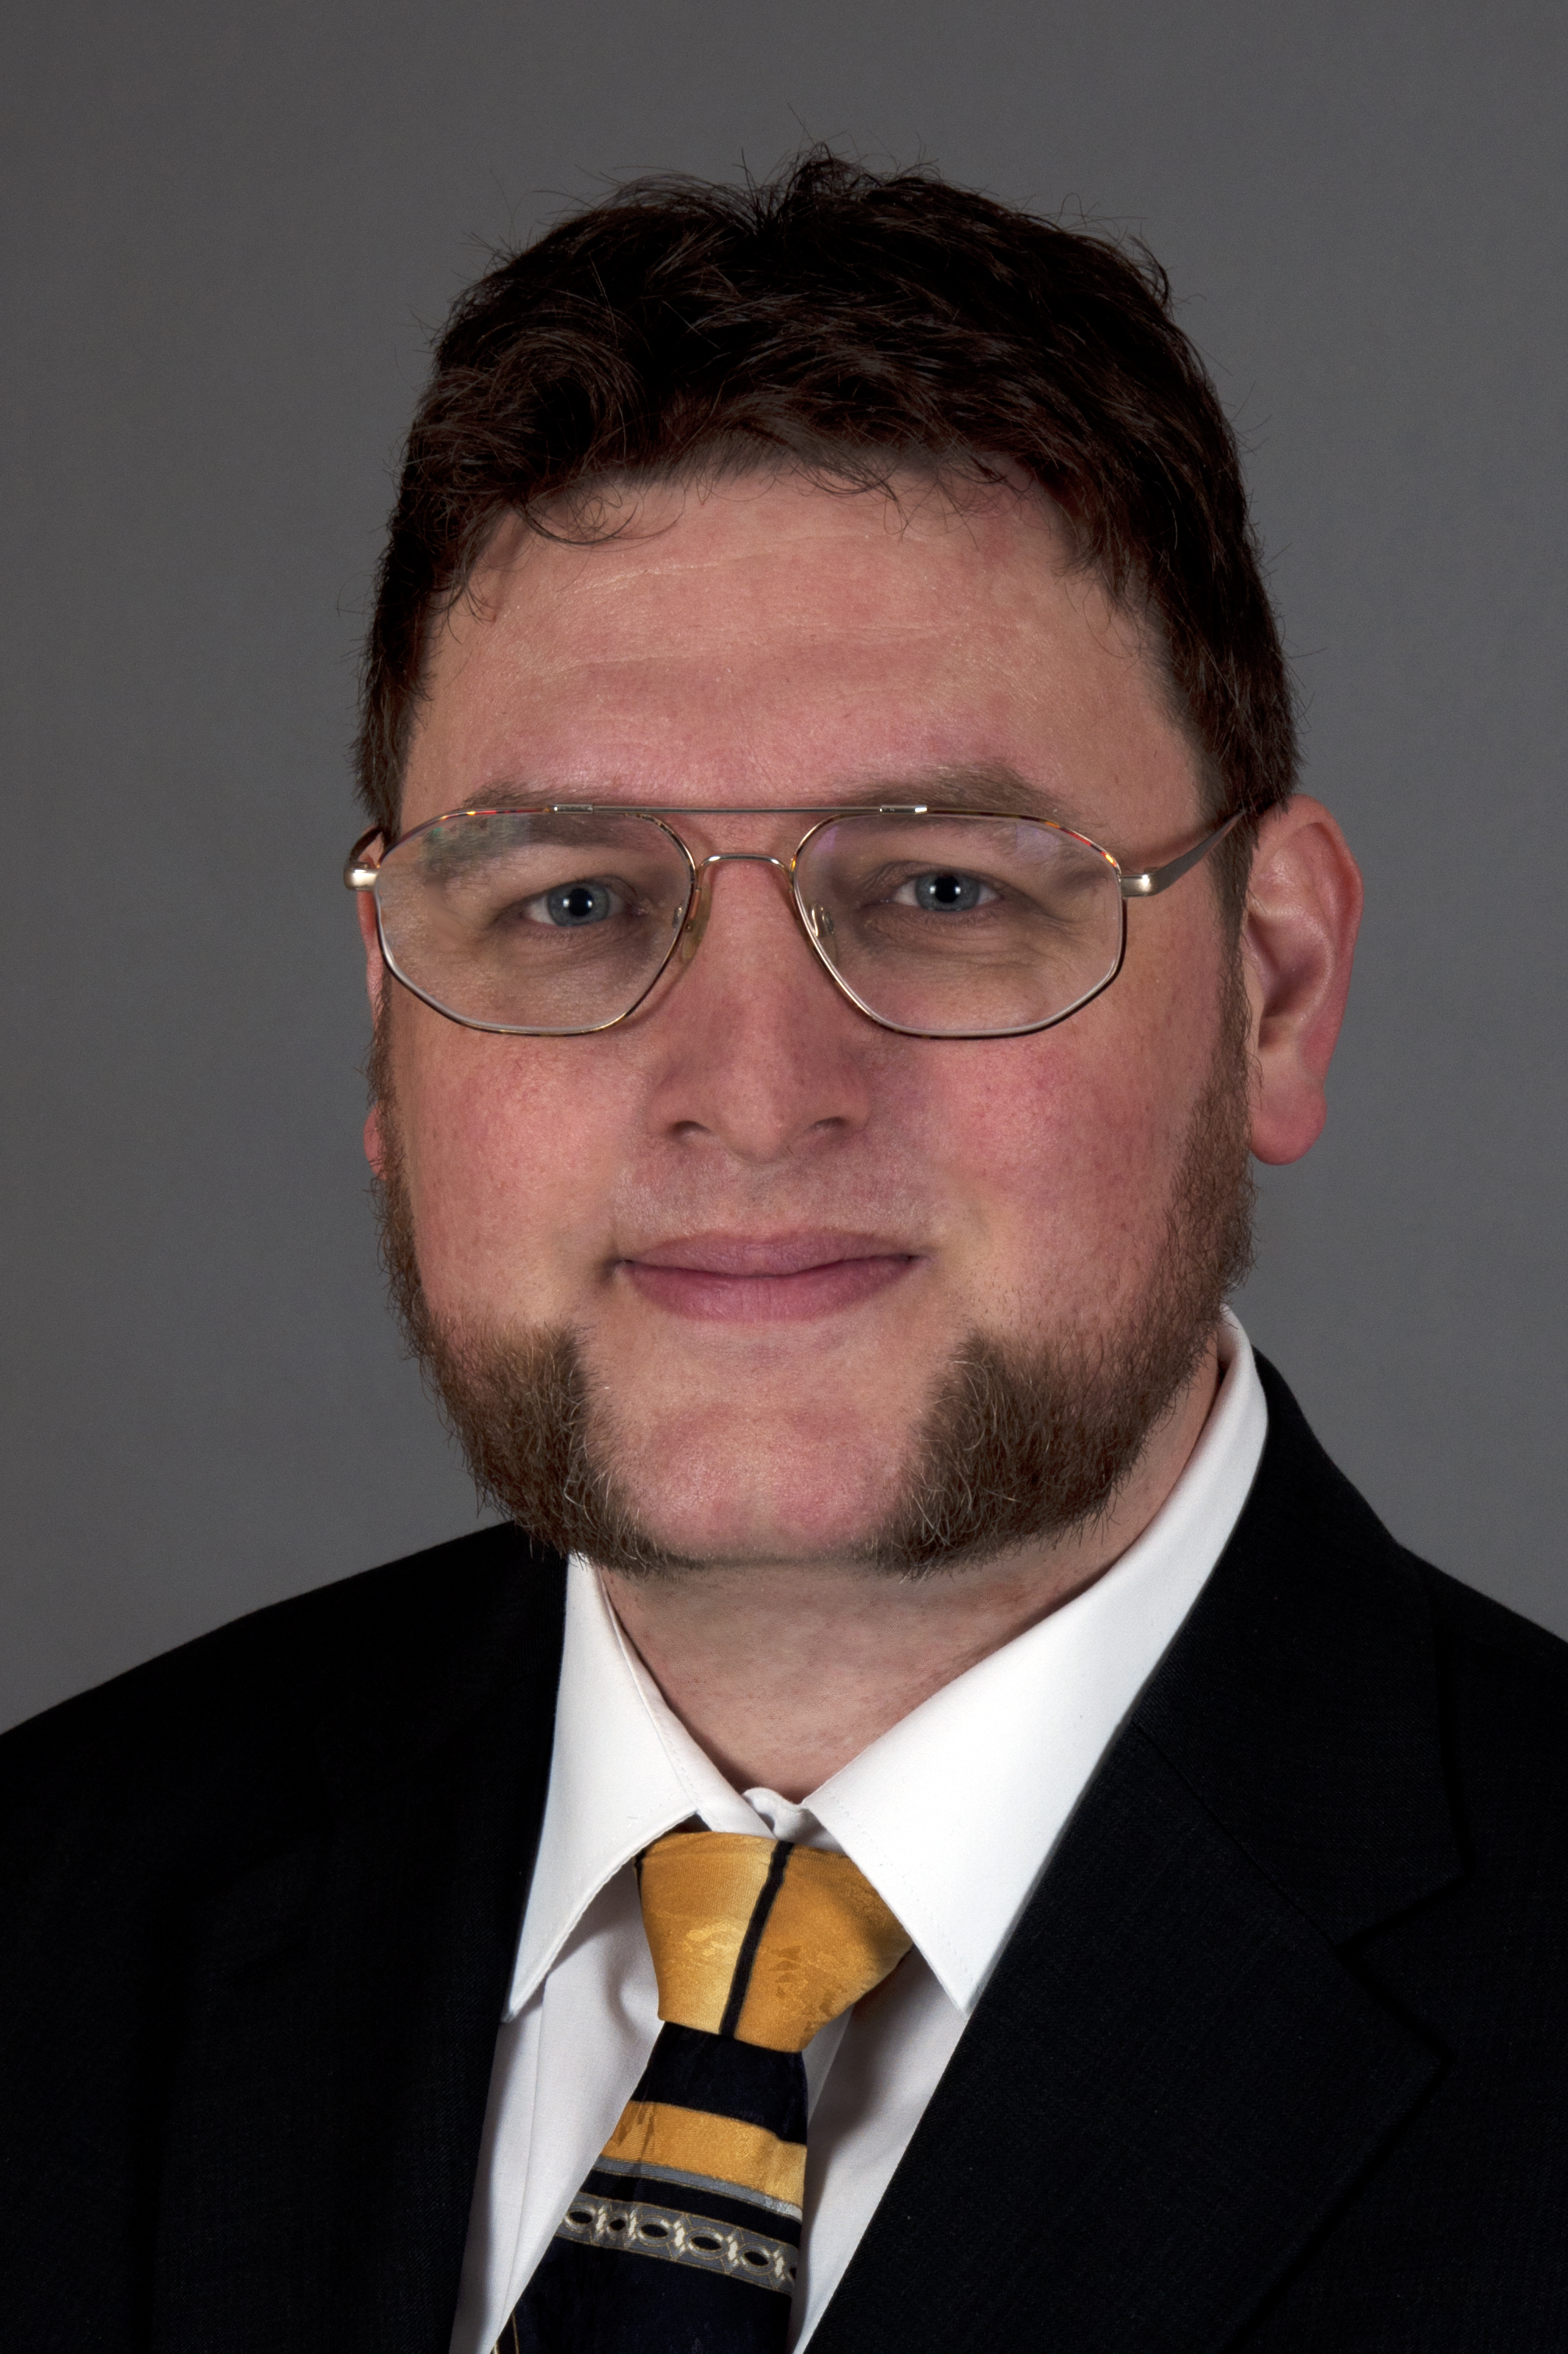
\includegraphics[width=0.29\columnwidth]{inc/biography/passphoto}
\end{wrapfigure}
% !TeX spellcheck = en_GB

Martin Gwerder was born 20. July 1972 in Glarus, Switzerland. He is currently a doctoral Student at the University of Basel. After having concluded his studies at the polytechnic at Brugg in 1997, he did a postgraduate study as a master of business and engineering. Following that, he changed to the university track doing an MSc in Informatics at FernUniversit\"at in Hagen. While doing this he constantly broadened his horizon by working for industry, banking and government as  engineer and architect in security related positions. He currently holds a lecturer position for cloud and security at the University of Applied Sciences Northwestern Switzerland. His main expertise lays in the field of networking related problems dealing with data protection, distribution, confidentiality and anonymity.

\begin{comment}
\section*{Personal Details}
\begin{tabular}{ll}
Name:             	& Martin Gwerder\\
Employer address: 	& Untere Parkstrasse 9,5212 Hausen AG, Switzerland\\
Email: 				& martin.gwerder@fhnw.ch\\
\end{tabular}
\section*{Career Summary}
Martin Gwerder started off with an apprenticeship as an electro mecanic. After concluding studies at the polytechnic he worked first as an engineer, later as seniorengineer, and architect for several companies in banking, industry and for the gvernment. 

\section*{Education}
Martin Gwerder is currently a doctoral Student at the University of Basel. After having concluded his studies at the polytechnic at Brugg in 1997, he did a postgraduate study as a master of business and engineering. Following that, he changed to the university track doing an MSc in Informatics at FernUniversit\"at in Hagen.

\section*{Focus}
The main focus of Martin Gwerder are in the fields of data protection, privacy, confidentiality, and anonymity.

\fxfatal{more content to CV}
\end{comment}

\end{document}
